
\documentclass[11pt]{book}
%usepackage[italian]{babel}
\usepackage{epsfig}
%\usepackage{psfig}
\usepackage{amssymb}
\usepackage{latexsym}
\usepackage{longtable}
\usepackage{subfigure}
\usepackage{graphics}
\usepackage{lscape}
\usepackage{a4wide}

\usepackage{graphicx}
\usepackage{natbib}


\newcommand{\msun}{M$_{\odot}$}
\newcommand{\kms}{km s$^{-1}$}

\begin{document}
\begin{titlepage}
\title{{\Huge The MANGA Data Analysis Pipeline: \\
a prototype}}
\author{L. Coccato \& MANGA team}
\end{titlepage}

\maketitle
\tableofcontents

% ======================================================================
%\newcommand{\kms}{km s$^{-1}$}
%\chapter{Introduction}
%\label{dap}
%
%
%\section{Abstract}
%\label{dap_sec:abstract}%
%
%This chapter %
%
%\subsection{Acronyms and definitions}%
%
%In this chapter, we will adopt the following acronyms and definitions:
%
%\begin{tabular}{l l}
%DRP & Data Reduction Pipeline \\
%DAP & Data Analysis Pipeline \\
%LOSVD & Line Of Sight Velocity Distribution \\
%LSF & Line Spread Function \\
%SRD & Sciente Requirement Document \\
%
%
%\end{tabular}




\chapter{Introduction}
\label{dap_chap:introduction}


\section{Data Analysis Pipeline (DAP): overview}
\label{dap_sec:dap_overview}

The scope of the Data Analysis Pipeline is to analyse the output of
the Data Reduction Pipeline and deliver science products. They are
classed into two groups, the {\bf High level data products} and the
{\bf Model dependent data products}.

High level data products are:
\begin{itemize}
     \item Stellar kinematics (velocity, velocity dispersion, h3, and h4 Gauss-Hermite moments).
     \item Emission line kinematics (velocity, and velocity dispersion).
     \item Equivalent widths and fluxes of emission lines.
     \item Absorption line strengths.
     \item Reddening.
     \item Radial gradients of measured quantities.
     \item Rotation curves and kinemetric parameters.
     \item Radial profiles of $\lambda$, $V/\sigma$, and $\sigma$.
     \item Stellar weights from full spectral fitting.
\end{itemize}

Model dependent data products are:
\begin{itemize}
    \item Stellar population parameters age, metallicity, chemical
      element ratios, and IMF, and their radial gradients (from absorption features).
    \item Stellar population parameters age, metallicity, chemical
      element ratios, and IMF, and their radial gradients (from full spectral fitting).
    \item Extinction corrected star formation rates and hystories.
    \item Gas metallicities, BPT diagrams.
    \item Mass to light ratio (from stellar population).
    \item Mass to light ratio, dynamical mass (from dynamical
      modeling).
    %\item Angular momentum.
   % \item Characterization of asymmetries, see Section \ref{sec:dynamical_state}.
   % \item Measurements of the Toomre Q-parameter, see Section  \ref{sec:growth_bulges}.
\end{itemize}%

\subsection{Installation and requirements}
\label{dap_sec:installation}
T.B.D.

\section{DAP workflow description}
\label{dap_sec:dap_workflow}

The DAP is divided into parts and blocks, the first part (blocks 1-6)
will deliver the High Level Data products (see Figure
\ref{dap_fig:dap_workflow_1}), the second part (blocks 7-9) will
deliver the Model dependent data products (see Figure
\ref{dap_fig:dap_workflow_2}). 

Each block is responsable for a set of operations, such as reading
data, fitting the input spectra. The procedure that executes an
operation is called ``main module''. The main modules comunicates
between them and between the various blocks via other procedures,
which are called ``interface module''. The main and interfaces modules
can call other modules, which are called ``unitily modules''. The
interface module is therefore responsable to get input files from a
previous interface, convert them in a readable format readable for the
main module, collect the outputs of the main module and convert them
in a form readable for the next interface. In this way, it is
relatively easy to change the software responsible for a specific task
(i.e. replacing the main module responsible for the spectral fitting)
by chaning its interface.  Table \ref{dap_tab:modules} list a summary
of the blocks, interfaces and main modules distribution.


\begin{table}
\begin{scriptsize}
\caption{Summary of blocks, interfaces and main modules distribution.}
\begin{tabular}{l |l |l | l}
BLOCK         & Interface modules               & Main  modules    & Utility modules   \\
\hline
\hline
%{\bf Block 1} &                                 &                                \\  
              &                                 &                               &  \\  
{\bf Block 1} & mdap\_read\_datacube            & mdap\_calculate\_spectrum\_sn  &    \\
\hline
%{\bf Block 2} &                                 &                                \\  
              &                                 &                             &\\  
{\bf Block 2} & mdap\_spatial\_binning          & mdap\_voronoi\_2d\_binning  & mdap\_calibrate\_sn   \\
 \hline
%{\bf Block 3} &                                 &                                \\  
              &                                 &                            &    \\  
{\bf Block 3} & mdap\_log\_rebin$^{1}$          & mdap\_do\_log\_rebin        & mdap\_convol\_sigma   \\
\hline
%{\bf Block 4} &                                 &                                \\  
              &                                 &                           &   \\  
{\bf Block 4} & mdap\_spectral\_fitting        & mdap\_calculate\_spectrum\_sn  & mdap\_range.pro \\
              & mdap\_create\_starting\_guesses & mdap\_bvls(\_external)        & mdap\_stc.pro \\
              &                                 & mdap\_dust\_calzetti          & mdap\_sgn.pro \\
              &                                 & mdap\_get\_losvd              & mdap\_round\_str.pro \\
              &                                 & mdap\_gandalf\_wrapf$^{2}$     & mdap\_interpolate\_2dmaps \\
              &                                 & mdap\_gandalf$^{2}$            & mdap\_ppxf\_convol\_fft \\
              &                                 & mdap\_ppxf$^{2}$               &  \\
              &                                 &{\tt mpfit package}              &  \\ 
\hline
%{\bf Block 5} &                                 &                                         \\  
              &                                 &                                         & \\  
{\bf Block 5} & mdap\_measure\_indices          & mdap\_read\_indices\_definitions$^{3}$  & mdap\_round\_str.pro \\
              &                                 & mdap\_do\_measure\_index               &  mdap\_convol\_sigma  \\
\hline
%{\bf Block 6} &                                 &                                         \\  
              &                                 &                                        &   \\  
{\bf Block 6} & mdap\_spatial\_radial\_binning  & mdap\_calculate\_spectrum\_sn       &  mdap\_convol\_sigma   \\
              & mdap\_spectral\_fitting       &   mdap\_do\_measure\_index            & mdap\_get\_losvd     \\ 
              & mdap\_measure\_indices          &   mdap\_dust\_calzetti             & mdap\_range.pro  \\
              &                                 &   {\tt mpfit package}              &  mdap\_stc.pro \\
              &                                 &   mdap\_sgandalf                   & mdap\_sgn.pro  \\
              &                                 &   mdap\_gandalf\_wrapf$^{2}$       &  mdap\_interpolate\_2dmaps \\
              &                                 &   mdap\_gandalf$^{2}$               & mdap\_read\_indices\_definitions$^{3}$\\
              &                                 &   mdap\_ppxf$^{2}$                  & mdap\_ppxf\_convol\_fft\\
              &                                 &   mdap\_bvls(\_external)         &  \\
\hline
              &                                 &  &  \\  
{\bf Block 7} &                                 &                                &  \\
\hline
              &                                 &  &  \\  
{\bf Block 8} &                                 &                                &  \\
\hline
              &                                 &  &  \\  
{\bf Block 9} &                                 &                                &  \\
\hline
\hline
\end{tabular}
\end{scriptsize}
\begin{minipage}{15cm}
Notes: 
$^{1}$ Need auxiliary files: stellar templates. 
$^{2}$ Need auxiliary file: Emission lines definitions. 
$^{3}$ Need auxiliary file: Absorption line index definitions.
\end{minipage}
\label{dap_tab:modules}
\end{table}

The input datacube is read in block 1 and information (vectors with
galaxy spectra, errors, wavelenght, and spatial information) are
passed to the block 2 for spatial binning. Three spatial binnings are
foreseen, depending on the scientific requirements. The current DAP
version uses the Voronoi binning scheme, (as implemented in IDL by
Cappellari \& Copin 2003), as main module for the spatial binning
task.

Binned spectra are passed to block 3 for logarithmic resampling of the
galaxy spectra (and error) and the stellar templates. Stellar
templates are also broadened to match the instrumental set up. For
this, the instrumental $LSF(\lambda)$ is required as input. Three sets
of log-sampled galaxy spectra are produced, one set for each spatial
binning.

The log-sampled spectra are then passed to block 4 for spectroscopic
measurements. Three fits are performed in block 4, one for each
spatial sampling defined in block 2. Before each fit, the log-sampled
Galaxy spectra are corrected for Milky Way extinction(input
parameter). Results from the first execution will be used to constrain
the fit of the second fit, and soforth. The current version uese: i)
the pPPXF.pro and gandalf.pro (Cappellari \& Emsellem 2004; Sarzi et
al. 2006); and ii) Calzetti et al. (2000) formulas for reddening
correction as main modules in block 4 (See Section
\ref{dap_sec:mdap_spectral_fitting} for further details). Fitting
procedures have been modified to allow the use of external fortran
routine, instrumental velocity dispersion variable with wavelength,
and fitting parameter boundaries from user input.

The output of block 4 are the kinematic
parameters of stars and gas, emission lines fluxes and equivalent
width, reddening, the weights of the stellar templates used in the fit
(for stellar population measurements), and rest-framed galaxy spectra.

Input galaxy spectra (with best-fit emission lines removed) will be
passed to block 5 for measurement of the line strenght. The current
design foresees that absorption line strength will be measured only
onto spectra associated to the first spatial binning (i.e. those with
the higher $S/N$. The current version uses the absoprtion line indices
as defined by Worthey et al. (1994).

Rest-framed spectra, Kinematic measurements, emission line fluxes,
absorption and emission line equivalent widths are then passed to
block 6 for the extraction of the radial profiles of the measured
quantities, and kinemetric analysis.

\subsection{DAP inputs and outputs}
\label{dap_sec:dap_inputs_outputs}

The Data Analysis Pipeline consists in a IDL procedure,
manga\_dap.pro, and a set of ``interfaces'' modules, ``main'' modules,
and ``utilities'', which are described in this document.

To run the pipeline, the following files are needed.
\begin{itemize}

\item total\_filelist.dat. This is the file that specifies the
  galaxies to analyse and their properties. The file must contain 5
  columns. The first column indicates the names of the $N$ datacubes
  (stored in .fits file, see Section
  \ref{dap_sec:mdap_read_datacube}), the second column provides an
  estimate of the galaxy redshift (in km/sec), the third column
  provides an estimate of the stellar velocity dispersion (in km/sec),
  the 4th column provides the mean galaxy ellipticity, and the 5th
  column provides the mean galaxy position angle.

\item all the $N$ files (datacubes or rss) listed in the file total\_filelist.dat.

\item a set of stellar templates, in fits file format.

%\item emission\_lines\_setup\_with\_Balmer\_decrement. A file containing the definitions of the emission lines to include in the fit (see Section \ref{dap_sec:mdap_spectral_fittig}).

%\item absorption\_line\_indices\_definition.dat. A file containing the definitions of the absorption line indices to measure (see Section \ref{dap_sec:mdap_measure_indices}). 
\item A file containing the definitions of the emission lines to include in the fit (see Section \ref{dap_sec:mdap_spectral_fittig}).

\item A file containing the definitions of the absorption line indices to measure (see Section \ref{dap_sec:mdap_measure_indices}). 

\item A configuration file, that contains all the parameters needed in the analysis.
\end{itemize}

The DAP is executed by the following IDL command line 

\[
{\tt IDL> manga\_dap,i,configuration\_file}
\]

where {\tt i} is the index number of the $i$-th entry in the
total\_filelist.dat, column 1 to analyse, $i=0,
N-1$. configuration\_file is a string specifying the name of the
configuration file. For a full description of the configuration file,
see Section \ref{dap_sec:configuration}.


As output, the DAP returns a multilayer fits file with all the
measured quantities (({\tt <datacube\_name> \_high\_level.fits}), an
idl session with all the session variables stored ({\tt
  <datacube\_name>\_mdap\_ session.idl}).  and a log file
(<datacube\_name>\_mdap.log).

The content of the {\tt <datacube\_name>\_high\_level.fits} output
file is described in Table \ref{dap_tab:output}.


\begin{center}
\begin{longtable}{p{0.5cm}|p{3.5cm}| p{10.1cm}}
\caption{Extension description of the DAP output fits file.} \label{dap_tab:output} \\
\hline
{\bf Ext} &  {\bf Name} &{\bf Description} \\
\hline
\endfirsthead
\hline
{\bf Ext} &  {\bf Name} &{\bf Description} \\
\hline
\endhead
\hline
\endlastfoot
\hline
%{\bf Ext} &  {\bf Name} &{\bf Description} \\
0 & signal              & Mean signal per pixel, produced by mdap\_read\_datacube.pro (Section \ref{dap_sec:mdap_read_datacube}). \\
1 & noise               & Mean noise per pixel, produced by mdap\_read\_datacube.pro (Section \ref{dap_sec:mdap_read_datacube}).\\
2 & binning map 1       & Location and geometry of the spatial bins of the first binning scheme.\\ 
3 & binning 1 data      & Measurements performed on the first binning scheme (absorption line indices).\\ 
4 & binning map 2       & Location and geometry of the spatial bins of the second binning scheme.\\ 
5 & binning 2 data      & Measurements performed on the second binning scheme (stellar kinematics). \\ 
6 & binning map 3       & Location and geometry of the spatial bins of the third binning scheme.\\ 
7 & binning 3 data      & Measurements performed on the third binning scheme (gas kinematics and emission line properties).\\ 
8 & binning map radial  & Location and geometry of the radial binning scheme.\\ 
9 & binning radial data & Measurements performed on the radial binning scheme (absorption line indices and stellar velocity dispersion).  \\ 
10 & Stars rotation & Kinemetric measurements on the stellar kinematics (kinematic position angle, rotation curve, inflows/outflows).  \\ 
11 & Gas rotation   & Kinemetric measurements on the gas kinematics (kinematic position angle, rotation curve, inflows/outflows).  \\ 
\hline
\end{longtable}
\end{center}

\subsubsection{Extension 3: outputs related to the first binning
  scheme} 
\label{}
The quantities measured and stored using the first binning scheme are
the following:

\begin{itemize}

\item Column 1. X. The X coordinates (in arcsec) of the centers of the spatial bins. The center of the field of view has coordinates (0,0).
\item Column 2. Y. The Y coordinates (in arcsec) of the centers of the spatial bins. The center of the field of view has coordinates (0,0).
\item Column 3. AREA\_BIN. Area in arcsec$^2$ of the spatial bin.
\item Column 4. STON. Estimate of the S/N of the spectrum in the
  spatial bin. The signal is defined as the median of the best fit
  model, the noise as the robust\_sigma of the residuals (observed
  spectrum - best fit).
\item Column 5. NELEMENTS. Number of spectra coadded in the spatial bin.
\item Columns 6-end. Equivalent width of the absorption line indices
  and their errors (Units \AA\ or magnitudes, depending on the index
  definition. The measured indices (and their names) are defined in a
  user-provided file. The name of this file is specified in the
  configuration file (see Section \ref{dap_sec:configuration}).
\end{itemize}

\subsubsection{Extension 5: outputs related to the second binning
  scheme} 
\label{}
The quantities measured and stored using the second binning scheme are
the following:

\begin{itemize}

\item Column 1. X. The X coordinates (in arcsec) of the centers of the spatial bins. The center of the field of view has coordinates (0,0).
\item Column 2. Y. The Y coordinates (in arcsec) of the centers of the spatial bins. The center of the field of view has coordinates (0,0).
\item Column 3. AREA\_BIN. Area in arcsec$^2$ of the spatial bin.
\item Column 4. STON. Estimate of the S/N of the spectrum in the
  spatial bin. The signal is defined as the median of the best fit
  model, the noise as the robust\_sigma of the residuals (observed
  spectrum - best fit).
\item Column 5. NELEMENTS. Number of spectra coadded in the spatial bin.
\item Columns 6-7. VEL and VEL\_ERR. Measured stellar velocity and its error in km/sec.
\item Columns 8-9. DISP and DISP\_ERR. Measured stellar velocity dispersion and its error in km/sec.
\item Columns 10-11. H3 and H3\_ERR. Measured Gauss-Hermite moment of the stellar velocity distribution h3 and its error (Warning: the maximum range allowed in the
  fitting procedure is : $-0.4 < {\rm H3} < 0.4$).
\item Columns 12-13. H4 and H4\_ERR. Measured Gauss-Hermite moment of the stellar velocity distribution h4 and its error (Warning: the maximum range allowed in the
  fitting procedure is : $-0.4 < {\rm H4} < 0.4$).
\item Column 14. CHI2. Chi-squared from the fit.
\end{itemize}

\subsubsection{Extension 7: outputs related to the third binning
  scheme} 


The quantities measured and stored using the third binning scheme are
the following:

\begin{itemize}

\item Column 1. X. The X coordinates (in arcsec) of the centers of the spatial bins. The center of the field of view has coordinates (0,0).
\item Column 2. Y. The Y coordinates (in arcsec) of the centers of the spatial bins. The center of the field of view has coordinates (0,0).
\item Column 3. AREA\_BIN. Area in arcsec$^2$ of the spatial bin.
\item Column 4. STON. Estimate of the S/N of the spectrum in the
  spatial bin. The signal is defined as the median of the best fit
  model, the noise as the robust\_sigma of the residuals (observed
  spectrum - best fit).
\item Column 5. NELEMENTS. Number of spectra coadded in the spatial bin.
\item Columns 6-7. VEL and VEL\_ERR. Flux-weighted mean velocity of the emission lines and its error in km/sec.
\item Columns 8-9. DISP and DISP\_ERR. Flux-weighted mean velocity dispersion of the emission lines and its error in km/sec.
\item Columns 10-11. E(B-V) color excess for the stellar component and its error
\item Columns 12-13. E(B-V) color excess for the ionized gas stellar component and its error
\item Column 14.  CHI2. Chi-squared from the fit.
\item Columns 15-end. Flux, flux error, Equivalent widths, and
  equivalent width errors of the emission lines.  The measured
  emission lines (and their names) are defined in a user-provided
  file. The name of this file is specified in the configuration file
  (see Section \ref{dap_sec:configuration}).
\end{itemize}

\subsubsection{Extension 9: outputs related to the radial binning
  scheme} 


The quantities measured and stored using the radial binning scheme are
the following:

\begin{itemize}

\item Column 1. AMAJ. Lenght of the semi-major axis (in arcsecs) describing the elliptical bin. AMAJ=0 is the center of the field of view.
\item Column 2. AMAJ\_LO. Lower limit boundary (in arcsec) of elliptical bin.
\item Column 3. AMAJ\_UP. Upper limit boundary (in arcsec) of elliptical bin.
\item Column 4. STON. Estimate of the S/N of the spectrum in the
  spatial bin. The signal is defined as the median of the best fit
  model, the noise as the robust\_sigma of the residuals (observed
  spectrum - best fit).
\item Columns 5-6.  DISP and DISP\_ERR. Measured stellar velocity dispersion and its error in km/sec.
\item Column 7.  CHI2. Chi-squared from the fit.
\item Columns 8-end. Equivalent width of the absorption line indices
  and their errors (Units \AA\ or magnitudes, depending on the index
  definition. The measured indices (and their names) are defined in a
  user-provided file. The name of this file is specified in the
  configuration file (see Section \ref{dap_sec:configuration}).
\end{itemize}

\subsubsection{Extension 10 (11): outputs related to the kinemetric analysis of stellar (gas) kinematics}
The quantities measured and stored in extension 10 (11) are:
\begin{itemize}
\item Column 1. Elliptical semimajor axis (computed fixing the systemic velocity and the kinematic center, position angle, and axial ratio).
\item Column 2. Mean kinematic position angle.
\item Column 3. Standard deviation of the kinematic position angles at each semimajor axis.
\item Column 4. Mean kinematic axial ratio.
\item Column 5. Standard deviation of the kinematic axial ratios at each semimajor axis.
\item Column 6. Systemic velocity.
\item Column 7. Standard deviation of the systemic velocities at each semimajor axis.
\item Column 8. Rotation velocity measured at each semimajor axis.
\item Column 9. Error on the rotation velocity measured at each semimajor axis.
\item Column 10. Expansion velocity measured at each semimajor axis.
\item Column 11. Error on the expansion velocity measured at each semimajor axis.
\item Column 12. X coordiante of the assumed center of rotation (0,0 is the center of the field of view).
\item Column 13. Y coordiante of the assumed center of rotation (0,0 is the center of the field of view).

\end{itemize}



See Section \ref{dap_sec:mdap_do_kinemetry} for more information on how these quantities are computed.



\section{The configuration file}
\label{dap_sec:configuration}

The configuration file defines variables and parameters used in the
DAP. No empty lines should be present, commented lines are marked with
'\#'. The content of the configuration file is the following:

\begin{itemize}

 \item total\_filelist. A string indicating the full path to the file
   listing the galaxies to analyze and their physical parameters (See
   Section \ref{dap_sec:dap_inputs_outputs}).

 \item datacube\_root\_dir. Path indicating the location of the data
   to analyse. Files in datacube format must be stored in
   $<$datacube\_root\_dir$>$\textbackslash datacubes; files in RSS
   format must be stored in $<$datacube\_root\_dir$>$\textbackslash
   rss.
 
 \item output\_root\_dir. Path indicating where the results of the
   analysis should be stored. The directories
   $<$output\_root\_dir$>$\textbackslash resuts\_datacubes, and
   $<$output\_root\_dir$>$\textbackslash resuts\_rss must exist.

 \item w\_range\_for\_sn\_computation. Two elements array that
   specifies the wavelength range where to compute the signal to noise
   ratio. This array is passed to the main module
   mdap\_read\_datacube.pro, via the optional input {\tt lrange} (See
   Section \ref{dap_sec:mdap_read_datacube}). The suggested vaue for
   MANGA is to adopt the r-gunn FWHM bandpasse, centered at the
   effective wavelength (i.e.  $5560.00 < \lambda < 6942.00$
   \AA\ Fukugita et al. 1998). Leave it undefined to use the entire
   spectral range.


 \item w\_range\_for\_sn\_computation\_for\_gas. Two elements array
   that specifies the wavelength range where to compute the signal to
   noise ratio for emission line science. This range will be
   redshifted accordingly to the galaxy systemic velocity (from the
   starting guesses). If not specified, the default option will be
   adopted, i.e. use the same wavelenght range (with no redshift
   correction) for continuum and emission line science. One possible
   suggestion is to use the $6530 < \lambda <6600$ wavelength range,
   which embraces H$\alpha$ and NII emission lines.

  \item trim\_wav\_range\_spatial\_binning\_1. Two elements vector
    specifying the wavelength region to analyse in the first spatial
    binning (units: \AA). Binned galaxy spectra (of the first spatial
    binning) will be trimmed accordingly, templates will be trimmed
    over a sligtly larger wavelenth range.  Its value is passed to the
    main module mdap\_log\_rebin, during the rebinning and trimming of
    the spectra in the first spatial binning scheme through the
    optional input wave\_range (See Section
    \ref{dap_sec:mdap_spatial_binning}). If not defined, the entire
    available wavelength range will be used.


  \item trim\_wav\_range\_spatial\_binning\_2. As above, but for the
    second spatial binning scheme (3 spatial binning schemes are
    foreseen in the DAP, see Section \ref{dap_sec:block2}, plus a
    radial binning scheme \ref{dap_sec:block6}).

  \item trim\_wav\_range\_spatial\_binning\_3. As above, but for the
    third spatial binning scheme (3 spatial binning schemes are
    foreseen in the DAP, see Section \ref{dap_sec:block2}, plus a
    radial binning scheme \ref{dap_sec:block6}).

  \item trim\_wav\_range\_radial\_binning. As above, but for the
    radial spatial binning scheme (3 spatial binning schemes are
    foreseen in the DAP, see Section \ref{dap_sec:block2}, plus a
    radial binning scheme \ref{dap_sec:block6}).


  \item velscale. Float value indicating the velocity scale to adopt
    for the logarithmic rebinned spectra (units km/sec/pixel). This
    value is passed to mdap\_log\_rebin via the keyword
    input\_velscale (see Section \ref{dap_sec:mdap_log_rebin}), and to
    mdap\_spectral\_fitting via the velscale input variable (see
    Section \ref{dap_sec:mdap_spectral_fitting}). The default is to
    use the one automatically defined by the input galaxy
    specta. Suggested value: 30 km/sec/pixel.

  \item stellar\_library\_spatial\_binning\_1. String specifying the
    path. Warning: files are identified with the IDL function {\tt
      file\_search(stellar\_library\_spatial\_binning\_1)}. Therefore,
    be sure that this is enough to identify all and only the files
    that are needed. Warning: stellar\_library\_spatial\_binning\_1
    will be used also for the radial binning scheme. Files in the
    library must be fits files covering a wavelenght range
    preferentially larger than the MANGA ($3000< \lambda <
    10000$). They must have an uniform angstrom/pixel sampling. The
    following header keywords need to be present: CRVAL1 (value at
    reference pixel), CRPIX1 (reference pixel), and CDELT1 (dispersion
    in angstrom/pixel). stellar\_library\_spatial\_binning\_1 is
    required, and it will be passed to the interface mdap\_ log\_rebin
    and via the library input variable.

  \item stellar\_library\_spatial\_binning\_2 Same as
    stellar\_library\_spatial\_binning\_1, but for stars to be used
    with the spectra of the secon spatial binning.


  \item stellar\_library\_spatial\_binning\_3. Same as
    stellar\_library\_spatial\_binning\_1, but for stars to be used
    with the spectra of the third spatial binning.


  \item sn1\_rss. Float indicating the target signal-to-noise to adopt
    in the Voronoi binning scheme for RSS format data in the first
    spatial binning. This is mandatory and it will be passed to the
    interface mdap\_spatial\_binning via the min\_sn input variable
    (see Section \ref{dap_sec:mdap_spatial_binning}). Suggested entry
    = 15.

  \item sn2\_rss. Same of sn1\_rss, but for RSS format data in the
    first spatial binning. Suggested entry = 10.

  \item sn3\_rss. Same of sn1\_rss, but for RSS format data in the
    third spatial binning. Suggested entry = 5.

  \item sn1\_datacubes.  Same of sn1\_rss, but for datacube format
    data in the first spatial binning. Suggested entry = 40.

  \item sn2\_datacubes.  Same of sn1\_rss, but for datacube format
    data in the second spatial binning. Suggested entry = 25.

  \item sn3\_datacubes.  Same of sn1\_rss, but for datacube format
    data in the third spatial binning. Suggested entry = 15.

  \item sn\_thr\_tpl\_rss = 2. Threshold value for the S/N per
    angstrom each spectrum of RSS data format needs to have to be
    included in the analysis. S/N is computed over the wavelength
    range defined by the w\_range\_for\_sn\_computation variable (see
    above). Specra whose S/N are lower than this value will be
    discarded.Default = 0. To avoid any S/N threshold, set this
    variable to a very negative value (i.e. -100). Suggested value = 2

  \item sn\_thr\_str\_rss. Same as sn\_thr\_tpl\_rss, but for RSS
    format data in the second spatial binning scheme.  Suggested value
    = 2.

  \item sn\_thr\_ems\_rss. Same as sn\_thr\_tpl\_rss, but for RSS
    format data in the hird spatial binning scheme. Suggested value =
    2.

  \item sn\_thr\_tpl\_datacubes. Same as sn\_thr\_tpl\_rss, but for
    datacube format data in the first spatial binning scheme.
    Suggested value = 2.

  \item sn\_thr\_str\_datacubes.  Same as sn\_thr\_tpl\_rss, but for
    datacube format data in the second spatial binning scheme.
    Suggested value = 2.

  \item sn\_thr\_ems\_datacubes. Same as sn\_thr\_tpl\_rss, but for
    datacube format data in the third spatial binning scheme.
    Suggested value = 2.

  \item sn\_calibration\_rss. Calibration coefficients for RSS format
    files. Formula is specified in the mdap\_calibrat\_sn.pro
    function. If not defined no calibration will be used (seggested).
    sn\_calibration\_rss is passed to mdap\_spatial\_binnin.pro and
    mdap\_voronoi\_2d\_binning.pro via the sn\_calibration keyword


 \item sn\_calibration\_datacubes. Calibration coefficients for
   datacube format files. Formula is specified in the
   mdap\_calibrat\_sn.pro function, and it is given by the following
   expression:

   \[
    {\rm S/N_{REAL}} = \sum_{i=1,N} C_i \cdot \left( \frac{{\rm S/N_{ESTIMATED}}^{C_0}}{ \sqrt{{\rm N}_{\rm spax} }} \right)^{i-1} 
   \]

   where $C_i$ are the coefficients of sn\_calibration\_datacubes, and
   N$_{\rm spax}$ are the number of spaxels in that spatial bin.

   If sn\_calibration\_datacubes is not defined, the relation
   S/N$_{\rm REAL}$ = S/N$_{\rm ESTIMATED}$ is used. Suggested values
   for the MaNGA test run are: [1.1, 0.743865, 1.10317, --0.0106751,
     4.00892$\cdot$10$^{-5}$].

   Warning: Coefficient calibrations were not computed for optimally
   weighted binned spectra (i.e. do not use if weight\_for\_sn=1.)

   sn\_calibration\_datacubes is passed to mdap\_spatial\_binnin.pro
   and mdap\_voronoi\_2d\_ binning.pro via the sn\_calibration keyword
   (see Section \ref{dap_sec:mdap_spatial_binning}).

 \item weight\_for\_sn. If set to 0, the voronoi binning scheme uses
   the Modified Lyoid algorithm, and spectra belonging to the same
   spatial bin are added together with no weighting. If set to 1 the
   voronoi binning scheme uses an optimal weighting procedure (Signals
   and Errors is weighted by $S/N^2$), and spectra belonging to the
   same spatial bin are added with weights given by $S/N^2$. This
   value is passed to the interface mdap\_spatial\_binning.pro and the
   module mdap\_voronoi\_2d\_binning.pro via the keyword
   weight\_for\_sn (see Section
   \ref{dap_sec:mdap_spatial_binning}). If not defined, the default
   value (0) is used (no weights are applied). Warning: if the
   weighting is used, the suggested S/N calibration (see below) is not
   valid.

 \item user\_bin\_map\_spatial\_binning\_1. String specifying the fits
   file to be used to set the first spatial binning scheme. If
   provided, it will override the Voronoi binning scheme. Default: use
   the S/N to define the voronoi binning. Its value will be passed to
   the interface mdap\_spatial\_binning.pro via the keyword
   user\_bin\_map (see Section \ref{dap_sec:mdap_spatial_binning})

 \item user\_bin\_map\_spatial\_binnin\_2. Same as before, but for the
   second spatial binning scheme.

 \item user\_bin\_map\_spatial\_binnin\_3. Same as before, but for the
   third spatial binning scheme.

 \item emission\_line\_file\_spatial\_binnin\_1. String specifying the
   name of the file which defines the emission lines to be fitted in
   the first spatial binning and the fit set-up parameters (see
   Sections \ref{dap_sec:mdap_spectral_fitting} and
   \ref{dap_sec:mdap_gandalf}). Its value will be passed to the
   interface mdap\_spectral\_fitting.pro via the keyword
   emission\_line\_file (see Section
   \ref{dap_sec:mdap_spectral_fitting}).

 \item emission\_line\_file\_spatial\_binnin\_2. Same as before, but
   for the second spatial binning.

 \item emission\_line\_file\_spatial\_binnin\_3. Same as before, but
   for the third spatial binning.
    
 \item emission\_line\_file\_radial\_binning. Same as before, but for
   the radial binning.

 \item absorption\_line\_indices. String specifying the name of the
   file which defines the absorption line indices to measure. It must
   be an ascii file with 9 columns:

   \begin{itemize}

     \item Column 1. Integer. Unique ID number of the absorption line
       feature.

     \item Column 2.String. Unique name of the absorption line
       feature. This will define the name of the field in sctructure
       of the DAP results (i.e. the name must begin with a letter,
       special characters like comas or dots are not allowed).

     \item Columns 3-4. Float (units: \AA) Lower and upper values of
       the index passpand.

     \item Columns 5-6.  Float (units: \AA) Lower and upper values of
       the index blue pseudo-continuum.

     \item Columns 7-8.  Float (units: \AA) Lower and upper values of
       the index red pseudo-continuum.

     \item Column 9. String (accepted values are: ang or
       mag). Specifies the units (\AA\ or magnitudes) of the output.
 
    \end{itemize}
      
   absorption\_line\_indices must be defined, and it will be passed to
   the interface mdap\_ measure\_indices.pro and the utility
   mdap\_read\_indices\_definitions.pro via the
   absorption\_line\_indices input variable (see Sections
   \ref{dap_sec:mdap_measure_indice} and
   \ref{dap_sec:mdap_read_indices_definitions}).

   Indices will be measured only if their blue and red pesudo-continua
   bandpasses are included in the considered wavelength range. If not,
   their values are set to NaN, and their errors to 99 in the final
   output file.

  \item save\_intermediate\_steps. If set to 1 at the end of each
    block an idl session with all the current variables is
    saved. Default: 0 (suggested)

  \item remove\_null\_templates. If set to 1, the stellar templates
    that have null weight after the fiting of the first spatial bin
    will be rejected from the other fits. It is meaningful only if the
    libraries used for the other spatial binnings are the same of that
    used for the first spatial binning. Default: 0 Suggested value =
    1.

  \item external\_library. String indicating the location of fortran
    or C executables that will replace some of the IDL modules for
    speed purposes. If undefined, IDL routines will be used. The
    current DAP structure foresees the following two values, and
    mdap\_bvls.pro will be substituted by the mdap\_bvls\_external.pro
    routine:

    \begin{enumerate}

      \item external\_library= $<$mangadap$>$/external/F90\_32/ for 32
        bit machines;
 
      \item $<$mangadap$>$/external/F90\_64/ for 64 bit machines.

    \end{enumerate}

   Default: undefined (using internal routines). we suggest to define
   it and use external routines. The value of external\_library will
   be passed to the interface mdap\_spectral\_ fitting.pro via the
   keyword external\_library (if defined it will be used for all the
   spatial binning)

  \item spectra\_fittin\_parameters\_patial\_binning\_1. String array
    containing the additional inputs and keyword to be passed to the
    mdap\_spectral\_fitting.pro interface via the input keyword
    extra\_inputs (see Section \ref{dap_sec:mdap_spectral_fitting}) to
    be used to analyse the spectra of the first spatial binning.
    Suggested values: {\tt ['MOMENTS = 4', 'DEGREE = -1', 'MDEGREE =
        4']} Warning: variables will be defined via the IDL execute()
    function within the mdap\_spectral\_fitting.pro.

  \item spectra\_fittin\_parameters\_patial\_binning\_2. Same of
    before, but for the second spatial binning. Suggested value: {\tt
      ['MOMENTS = 4', 'DEGREE = -1', 'MDEGREE = 4']}

  \item spectra\_fittin\_parameters\_patial\_binning\_3.  Same of
    before, but for the third spatial binning. Suggested value: {\tt
      ['MOMENTS=4', 'MDEGREE=4', 'DEGREE=-1', 'reddening =
        [0.01,0.01]', 'LAMBDA = exp(loglam\_gal)']}

  \item spectra\_fittin\_parameters\_patial\_binning\_readial.  Same
    of before, but for the radial binning. Suggested value: {\tt
      ['MOMENTS=4', 'DEGREE=-1', 'mdegree=4', 'reddening = [0.01]',
        'LAMBDA = exp(loglam\_gal)']}

  \item instrumental\_fwhm\_file String indicating the name of the
    file with the wavelenght dependence of the instrumental FWHM. The
    file needs to be ascii with 4 columns.

  \begin{itemize}
     \item Column 1 : wavelength in angstrom, where the instrumental
       FWHM has been measured
     \item Column 2 : Resolving power.
     \item Column 3 : Instrumental FWHM in angstrom.
     \item Column 4 : Instrumental FWHM in km/sec.
  \end{itemize}

  Warning: Column 2 will not be used by the DAP, but it needs to be
  present to make the procedure running.

  If instrumental\_fwhm\_file is undefined, a constant instrumental
  FWHM of 2.54 \AA\ will be used.

\end{itemize}


\subsection{Version control and tags. Obsolete}
\label{dap_sec:dap_version}


At the beginning of the execution, the DAP check whether the output
.fits file and .idl sessions exist. If so, it reads the version(s)
used to generate the existing files. If the current module versions
are greater than those used to generate the output file, the analysis
is performed again.

\begin{itemize}

\item {\bf manga\_dap\_version}. The version of the DAP. If the module
  version is greater than that stored in the output files, the entire
  analysis is performed again (currently, blocks 1-5).

\item {\bf mdap\_read\_datacube\_version}. The version of modules in
  block 1. If it is greater than that stored in the output file, blocs
  1-5 are executed again.

\item {\bf mdap\_spatial\_binning\_version}. The version of modules in
  block 2. If it is greater than that stored in the output file, blocs
  2-5 are executed again. It must include version information about
  mdap\_voronoi\_binning.pro as well.

\item {\bf mdap\_log\_rebin\_version}. The version of modules in
  block 3. If it is greater than that stored in the output file, blocs
  3-5 are executed again.

\item {\bf mdap\_spectral\_fitting\_version}. The version of modules
  in block 4. If it is greater than that stored in the output file,
  blocs 4-5 are executed again. It must include version information
  about mdap\_sgandalf.pro as well.

\item {\bf mdap\_measure\_index\_version}. The version of modules in
  block 5. If it is greater than that stored in the output file, block
  5 is executed again.

\end{itemize}

Warning: the version control is enabled only if the keyword
/check\_version is set.

\begin{figure}
\begin{center}
%\hspace{-2cm}
%\includegraphics[width=6cm,angle=90]{dap_workflow_1.ps}  25 150 810 445
\psfig{file=figures/mangaDAP_workflow_1.ps, width=9.5cm, clip=, bb= 140 10 480 800}
%\vspace*{0cm}
\caption{Workflow chart of the Data Analysis Pipeline (High Level Data products).}
 \label{dap_fig:dap_workflow_1}
\end{center}
\end{figure}


\begin{figure}
\begin{center}
%\hspace{-2cm}
%\includegraphics[width=6cm,angle=90]{dap_workflow_1.ps}  65 144 702  420 
\psfig{file=figures/mangaDAP_workflow_2.ps,  width=9cm, clip=, bb= 22 20 340 800}
%\vspace*{0cm}
\caption{Workflow chart of the Data Analysis Pipeline (Model Dependent Data products).}
 \label{dap_fig:dap_workflow_2}
\end{center}
\end{figure}

\chapter{BLOCKs and ``interface'' modules}
\label{dap_chap:blocks}

\section{DAP Block 1: reading the input data}
\label{dap_sec:block1}

This block reads the input data (in the form of a datacube or RSS
files) and extracts the all information needed for further processing,
such as the galaxy spectra and errors, wavelength vector, 2D maps
containing the coordinates, and galaxy signal and noise. The interface
module in this block is: mdap\_read\_datacube.pro (see Section
\ref{dap_sec:mdap_read_datacube} for a list of inputs and outputs).


The origin of the reference coordiante system of the input datacube
(or RSS files) is set to be the center of the field of view. The
mdap\_read\_datacube.pro interface computes the center if the galaxy
and set the reference coordinate system to the galaxy center. The
galaxy center is computed via centroid fitting on the
signal2d\_reconstructed image via the gcntrd.pro IDL routine.

If the change of coordinates is larger than 3'' in $X$ or $Y$, the
galaxy center is automatically set to be the same of the field of
view. This is to avoid failures in the centroid fitting caused by the
presence of foregroud stars in the field of view.

The main modules in the block, called by the interface, are
mdap\_calculate\_spectrum\_sn.pro (see Section
\ref{dap_sec:mdap_calculate_spectrum_sn} for a list of inputs and
outputs).

The Block will provide the galaxy spectra (and errors),
two-dimensional maps with coordinates (in arcseconds, the center of
the field has coordinates 0,0), the two-dimensional maps of the signal
and the noise (per angstrom), the wavelength vector (in \AA) and
related quantities (initial \AA, reciprocal dispersion
\AA\ pixel$^{-1}$), and header information for 2-dimensional
maps. Figure \ref{dap_fig:block1} illustrates the flowchart of block
1.


\begin{figure}
\begin{center}
\psfig{file=figures/block1.ps, width=15.0cm, clip=}
\caption{Workflow chart of the block 1 of the Data Analysis
  Pipeline. See Section \ref{dap_sec:mdap_read_datacube} for a
  description of inputs and outputs.}
 \label{dap_fig:block1}
\end{center}
\end{figure}


\subsection{{\tt mdap\_read\_datacube.pro}}
\label{dap_sec:mdap_read_datacube}

This interface module reads the input datacube or RSS files (which
must be multi-layer fits file) and extract from it all the arrays and
quantities, which are needed for the analysis. Table
\ref{dap_tab:mdap_read_datacube} list the inputs and outputs required
for this module.



\begin{center}
\begin{longtable}{p{2.7cm}| p{11.1cm}}
\caption{Inputs and outputs parameters of mdap\_read\_datacube.pro} \label{dap_tab:mdap_read_datacube} \\
\hline
{\bf  INPUTS} & \\
\hline
\endfirsthead
\hline
\endhead
\hline
\endlastfoot
\hline
datacube\_name & string with the name of the fits file containing the input in datacube or RSS formats. 
                         For inputs in datacube format, the file must be a fits file with the following
                         extensions:
                                \begin{enumerate}
                             \item flux in 1e-17 ergs/s/cm$^{-2}$/\AA. This extension must be a 3D
                               array, with the wavelength direction along the 3rd axis. 
                            \item  Inverse variance associated to the first extension
                            \item  Wavelength solution (1D dbl array). Constant linear step
                              (preferred)? Constant Log-step? Constant ln-step?
                            \item  RSS format (row-stacked spectra) (NOT USED)                  
                            \item  coverage map; (NOT USED)
                           \end{enumerate}

                         For inputs in RSS format, the file must be a fits file with the following
                         extensions:
                          \begin{enumerate}
                            \item flux in 1e-17 ergs/s/cm$^{-2}$/\AA. This extension must be a 3D
                               array, with the wavelength direction along the 3rd axis.
 
                            \item Inverse variance associated to the first extension

                            \item Wavelength solution (1D dbl array). Constant linear step
                              (preferred)? Constant Log-step? Constant ln-step?
                            
                            \item X position table.  Since position is a function of wavelength this is an 
                               array of the same size as the flux array.  Coordinates should be in arcseconds 
                               relative to the center of the data cube (i.e., roughly the center of the galaxy).
                            \item Y position table.
                            \end{enumerate}\\
%
\hline
{\bf  OPTIONAL INPUTS}  & \\
\hline
lrange & [2 elem vector]. It indicates the wavelentgh range (in angstrom) where to
       extract the information for Signal and Noise. Default: use the entire
spectra range \\
%
\hline {\bf OPTIONAL KEYWORDS} &  \\ 
\hline 
/keep\_original\_ step & If set, the wavelength output vector will be the same as the one
                         define from the input fits file. The default
                         is to re-construct (and  therefore re-inrpolate the galaxy and error
                         spectra) the output wavelength vector with constant ang/pixel step
                         using the minimum ang/pixel step that is stored in the wavelength
                         solution. For MANGA, it is suggested to set this keyword.\\
%
\hline
{\bf  OUTPUTS} &  \\
\hline
data           &  Galaxy spectra. [NxMxT dbl array] in the case that the inputs are in datacube format, or [NxT dbl array]
               in the case the inputs are in RSS format. Spectra are resampled over the vector wavelength.    \\
%
error          & Errors associated to data. [NxMxT dbl array] in the case that the inputs are in datacube format, or [NxT dbl array]
               in the case the inputs are in RSS format. Spectra are resampled over the vector wavelength. \\
%
wavelength     & [T dbl array]. Wavalenght value where data and errors are computed. The vector is constructed with constant linear step in ang/pixel 
               (unless the $\backslash$keep\_original\_ step keyword is selected). If input spectra have a logarithmic sampling, 
               the minimum available step is used (e.g. log\_lam[1]-log\_lam[0]).   \\
%
x2d            & Array containing the x coordinates in arcseconds (0 is the center of the field of view). 
               [NxM dbl array] in the case that the inputs are in datacube format, or 
               [N dbl array] in the case the inputs are in RSS format. \\
%
y2d            & Array containing the y coordinates in arcseconds (0 is the center of the field of view). 
               [NxM dbl array] in the case that the inputs are in datacube format, or 
               [N dbl array] in the case the inputs are in RSS format. \\
%
signal         & Mean galaxy signal per \AA, obtained considering all the wavelength range 
               (or only the range specified by lrange).               
               [NxM dbl array] in the case that the inputs are in datacube format, or 
               [N dbl array] in the case the inputs are in RSS format. 
               The signal is computed as the median of each spectrum, in the wavelength range specified by lrange. \\
\\
%
noise          & Mean galaxy error per \AA, obtained considering all the wavelength range 
               (or only the range specified by lrange). Calculation is done on original spectra, not those resampled over the vector wavelenght.
               [NxM dbl array] in the case that the inputs are in datacube format, or 
               [N dbl array] in the case the inputs are in RSS format.
               The signal is computed as the median of each error, in the wavelength range specified by lrange.\\
%               
cdelt1         & [double].        Spatial sampling along x direction (arcsec/pixel). If inputs are in RSS format, it is set to 0.5.  \\
cdelt2         & [double].        Spatial sampling along y direction (arcsec/pixel). If inputs are in RSS format, it is set to 0.5.  \\
header2d       & [str array].     The header for output two-dimensional maps produced by the DAP. \\
\hline
{\bf  OPTIONAL OUTPUTS} &  \\
\hline
version & string specifying the module version. If requested, the module is not execute and only version flag is returned.\\
 x2d\_ reconstructed  &   [NxM array]   If input is in DATACUBE format, x2d\_ reconstructed = x2d.

                          [N'xM' array] If inputs are in RSS format, the x2d coordinates are resampled over a 2D map with fixed 0"5/pixel sampling
                                     and define the  x2d\_ reconstructed map.\\
%
 y2d\_ reconstructed &    [NxM array]   If input is in DATACUBE format, y2d\_reconstructed = y2d.

                          [N'xM' array] If inputs are in RSS format, the y2d coordinates are resampled over a 2D map with fixed 0"5/pixel sampling
                                     and define the  y2d\_ reconstructed map.\\
%
 signal2d\_ reconstructed  &  [NxM array]   If input is in DATACUBE format, signal2d\_reconstructed = signal.

                         [N'xM' array] If inputs are in RSS format, the signal is resampled over the 2D map defined by
                                         x2d\_ reconstructed  and y2d\_ reconstructed. \\
%
 noise2d\_ reconstructed  &   [NxM array]   If input is in DATACUBE format, noise2d\_reconstructed = noise.

                        [N'xM' array] If inputs are in RSS format, the noise is resampled over the 2D map defined by
                                         x2d\_reconstructed  and y2d\_reconstructed. \\
%
 version   & [string]            Module version. If requested, the module is not execute and only version flag is returned.\\
%
\hline
\end{longtable}
\end{center}


\subsubsection{Future developments}

The following items needs to be implemented:

\begin{itemize}
  \item Implement with new format of input datacube.
  \item Allow for identification and removal of foreground stars.
\end{itemize}



\section[DAP Block 2: Spatial binning]{DAP Block 2: Spatial binning}
\label{dap_sec:block2}

This block adds adjacent spectra in the field of view to reach a
minimum signa-to-noise ratio, and organizes the observations into
spatial bins. 

It requires the spectra, errors, signals and noise for each spectrum,
and the coordinates obtained from block 1 as inputs. It returns the
binned spectra (and errors) and all the geometrical information of the
spatial bin (2D maps and coordinates of the bins center). It handles
both datacubes and RSS input files format.

Three different spatial binning schemes with different
are handled, depending on the scientific purposes.


\begin{enumerate}

\item First binning, which requires a minimum $S/N = 40$ per
  \AA. The spectra binned this way will be used to measure the
  equivalent width ob absorption line indices, to perform the full
  spectral fitting, and to derive the stellar population properties.

\item Second binning, which requires a minimum $S/N = 25$ per
  \AA. The spectra binned this way will be used to measure the
  stellar kinematics and dynamical models.


\item Third binning, which requires a minimum $S/N = 15$ per
  \AA. The spectra binned this way will be used to measure the
  emission line kinematics, fluxes, and widths, the reddening, gas
  metallicities and star formation rates.

\end{enumerate}

$S/N$s are computed in the wavelength range $5560 < \lambda < 6942$
(SLOAN r-band).


The interface module in this block is mdap\_spatial\_binning.pro (see
Section \ref{dap_sec:mdap_spatial_binning}). The main module is
mdap\_voronoi\_2d\_binning.pro (Section
\ref{dap_sec:mdap_voronoi_2d_binning}).

mdap\_voronoi\_2d\_binning.pro uses an imlementation of the Voronoi
Binning technique developed by \citet{Cappellari+03} (see Section
\ref{dap_sec:mdap_voronoi_2d_binning}). The implementation accounts
for spatial correlation between errors of adjacent spectra: the
estimated $S/N$ is calibrated to the real $S/N$ via empirical relation
and it is done by the utility module mdap\_calibrate\_sn.pro.

Note that RSS spectra do not require the above $S/N$ calibration,
because the errors between adjacent RSS files are not correlated.


The interface mdap\_spatial\_binning.pro accepts an user-defined fits
file describing the spatial binning scheme. This file needs to be
provided via the input keyword: user\_bin\_map. The names are defined
in the DAP configuration file (see Section
\ref{dap_sec:configuration}). The inclusion of an used-defined file
overrides the Voronoi binning.

On request, the spectra in the same spatial bin can be added together
by weighting them with their $S/N^2$ (weight\_by\_sn keyword).

Figure \ref{dap_fig:block2} illustrates the flowchart of block 2.

\subsubsection{Future implementations}
Future implementations:

\begin{itemize}

 \item calculation of spatial covariance matrix to account for error
   correlations and avoid the use of $S/N$ calibration relations.

  \item Allow for an equal flux surface binning scheme (Sanchez et
    al. ?) instead of the Voronoi binning scheme.

\end{itemize}

\begin{figure}
\begin{center}
%\hspace{-2cm}
%\includegraphics[width=6cm,angle=90]{dap_workflow_1.ps}
\psfig{file=figures/block2.ps, width=16.0cm, clip=,bb=25 77 590 815}
%\vspace*{0cm}
\caption{Workflow chart of the block 2 of the Data Analysis
  Pipeline.}
 \label{dap_fig:block2}
\end{center}
\end{figure}

\subsection{{\tt mdap\_spatial\_binning.pro}}
\label{dap_sec:mdap_spatial_binning}

This module is an interface for the mdap\_voronoi\_2d\_binning.pro
module, which uses the Voronoi Binning scheme (modified Loyd
algorithm) to combine adjacent spectra in the field of view till a
minimum $S/N$ is reached (see Section
\ref{dap_sec:mdap_voronoi_2d_binning}).

If the minimum $S/N$ is not reached, the requirement will be
automatically decreased by a factor 0.7 till convergence. By default,
spectra with mean $S/N < 4$ per \AA will be discarded. At least, 1
spectrum per datacube will be produced.

If user-defined spatial binning is provided (via the user\_bin\_map
keyword) the Voronoi binning scheme is overrided.

Table \ref{dap_tab:mdap_spatial_binning} lists the inputs and outputs
required for this module.

\begin{center}
\begin{longtable}{p{2.7cm}| p{11.1cm} }
\caption{Inputs and outputs parameters of mdap\_spatial\_binning.pro} \label{dap_tab:mdap_spatial_binning} \\
\hline
\endfirsthead
\hline
\endhead
\hline
\endlastfoot
\hline
{\bf  INPUTS} & \\
\hline
data   &    Galaxy spectra as produced by mdap\_read\_datacube.pro.
           [NxMxT dbl array] if DATACUBE format or [NxT dbl array]if RSS format.\\
%
error  &    Errors associated to data, produced by mdap\_read\_datacube.pro.
           [NxMxT dbl array] if DATACUBE format or [NxT dbl array]if RSS format.\\
%
signal  &   Mean galaxy signal per \AA, produced by mdap\_read\_datacube.pro.
           [NxM dbl array] if DATACUBE format or [N dbl array]if RSS format.\\
%
noise  &    Mean galaxy error per \AA,  produced by mdap\_read\_datacube.pro. 
           [NxM dbl array] if DATACUBE format or [N dbl array]if RSS format.\\
%
min\_sn &    [float] Minimum S/N (per \AA) required for the output binned spectra.\\
%
x2d   &     Array containing the x coordinates in arcseconds (0 is the center of the field of view), produced by  mdap\_read\_datacube.pro.    
            [NxM dbl array] if DATACUBE format or [N dbl array]if RSS format.\\
%
y2d   &     Array containing the y coordinates in arcseconds (0 is the center of the field of view), produced by  mdap\_read\_datacube.pro.    
           [NxM dbl array] if DATACUBE format or [N dbl array] if RSS format.\\
%
stepx  &    [float] Scale arcsec/pixel along X direction, computed by  mdap\_read\_datacube.pro. \\
%
stepy   &   [float] Scale arcsec/pixel along Y direction, computed by  mdap\_read\_datacube.pro. \\
%
\hline
{\bf OPTIONAL INPUTS} & \\
\hline
%
sn\_thr   &  [float] If specified, spectra with S/N lower than this value will be excluded from the analysis. \\ 
%
x2d\_ reconstructed & [N'xM' array] Two-dimesional map of X coordinates where the output spatial\_binning should be created. Required and used only  
                    if the input data are in RSS format. \\
%
y2d\_ reconstructed & [N'xM' array] Two-dimesional map of Y coordinates where the output spatial\_binning should be created. Required and used only 
                    if the input data are in RSS format. \\
%
SN\_ CALIBRATION    & vector. If provided, the estimated signal-to-noise ({\tt SN\_est}) is converted into the real signal-to-noise ({\tt SN\_real}) using the empirical
                  calibration function defined in mdap\_calibrate\_sn.pro:
           \[
           {\rm S/N_{REAL}} = \sum_{i=1,N} C_i \cdot \left( \frac{{\rm S/N_{ESTIMATED}}^{C_0}}{ \sqrt{{\rm N}_{\rm spax} }} \right)^{i-1} 
            \]

                    where {\tt Nbin} is the number of spectra added in that spatial bin.\\
%
user\_bin\_map   &  string  If provided, the spatial map will be created
                      from the fits fiel specified by this input. The
                      fits file must contain the CRVAL1, CRVAL2,
                      CDELT1, CDELT2, NAXIS1, NAXIS2, CRPIX1, and
                      CRIX2 header keywords (coordinate units in
                      arcseconds, 0,0 indicates the center of the
                      field of view. \\

\hline
{\bf INPUT KEYWORDS} & \\
\hline
%
/plot        &       If set, some plots on X11 terminal will be shown. Not suggested if the task is launched remotely. \\
% 
/weight\_for\_sn & If set, the spectra in the same spatial bin will be
                 weighted by $S/N^2$ before being added. If The voronoi binning scheme
                 is adopted, the S/N in the bin is computed via equation (3) of
                 Cappellari \& Copin (2003) and the centers of te spatial bins are computed by
                 weighting spectra coordinates by $S/N^2$.\\ 
%
\hline
{\bf OUTPUTS} & \\
\hline
%
binning\_map & Two dimensional map showing the binning sheme. Pixels beloning to the i-th bin have value i (i=0, 1, ..., Nbins). 
             Pixels associated to no spatial bin have value -1.  
             [NxM dbl array] if inputs are in DATACUBE format or [N'xM' dbl array] if inputs are in RSS format (interpolated 
             over x2d\_reconstructed and y2d\_reconstructed).\\
%
spectra   &  [Nbins x T dbl array]    The binned spectra of the spatial Nbins. i-th spectrum is associated to the i-th bin. \\
%
errors    &  [Nbins x T dbl array]    Errors vectors associate do the binned spectra. \\
%
xNode     &  [Nbins elements array]   X-Coordinates in arcsec of the luminosity weighted centers of the spatial bins. \\
%
yNode     &  [Nbins elements array]   Y-Coordinates in arcsec of the luminosity weighted centers of the spatial bins. \\
%
area\_bins &  [Nbins elements array]   Area (in arcsec$^2$) of each spatial bin.  \\
%
bin\_sn   &  [Nbins elements array]   Mean S/N per \AA reached in each spatial bin. \\
%
\hline
{\bf OPTIONAL OUTPUTS} & \\
\hline
%
 nelements\_ within\_ bin & [Nbins elements array] number of spaxels (in the case of DATACUBE format) or number of fibres (in the case of RSS format) coadded in each spatial bin.\\
%
 version   & [string]            Module version. If requested, the module is not execute and only version flag is returned.\\
\hline
\end{longtable}
\end{center}




\section[DAP Block 3: Logarithmic sampling]{DAP Block 3: Logarithmic sampling of input galaxy spectra and stellar templates}
\label{dap_sec:block3}

This block is responsable for:

\begin{itemize}

\item resampling the input galaxy spectra and errors (rebinned
  spectra, input from block 2) to a ln-wavelength constant step.

\item resampling the stars in the spectral library in the same
  ln-wavelength constant step used for galaxy spectra, and ensuring
  that the stars have the same instrumental resolution (i.e. the same
  LSF) of the galaxy spectra.

\item selecting only the wavelength region of interest, making sure
  that the wavelenght range of the template stars is larger than that
  of the galaxy spectra.

\item defyning the wavelenght vectors (ln units) over which the galaxy
  spectra, galaxy errors, and template stars are defined.

\end{itemize}

Because the DAP performs three different spatial binnings of the input
galaxy, the block operates

The interface module in this block is mdap\_log\_rebin.pro (see
Section \ref{dap_sec:mdap_log_rebin}), which calls the main module
mdap\_do\_log\_rebin.pro that performs the logarithmic resampling (see
Section \ref{dap_sec:mdap_do_log_rebin}). Because the DAP performs
three different spatial binnings of the input galaxy, block 3 executes
mdap\_log\_rebin.pro three times, one for each set of spatially binned
spectra. The workflow of block 3 is shown in Figure
\ref{dap_fig:block3}.

The current version of the DAP uses the MARCS stellar library models
(Maraston \& Stromback, 2011, MNRAS, 418, 2785).

\begin{figure}
\begin{center}
%\hspace{-2cm} \includegraphics[width=6cm,angle=90]{dap_workflow_1.ps}
\psfig{file=figures/block3.ps, width=13.5cm, clip=,bb=30 70 592 790}
%\vspace*{0cm}
\caption{Workflow chart of the block 3 of the Data Analysis
  Pipeline.}
 \label{dap_fig:block3}
\end{center}
\end{figure}

\subsection{{\tt mdap\_log\_rebin.pro}}
\label{dap_sec:mdap_log_rebin}

This interface controls the main module is responsable for the
logarithmic resampling of the input galaxy spexctra, errors, and the
stellar templates. It also broadens the input stellar spectra to match
the galaxy instrumental resolution. 

The list of input/output parameters defined in mdap\_log\_rebin.pro is
given in Table \ref{dap_tab:mdap_log_rebin}.



\begin{center}
\begin{longtable}{p{2.7cm}| p{11.1cm}}
\caption{Inputs and outputs parameters of mdap\_log\_rebin.pro} \label{dap_tab::mdap_log_rebin} \\
\hline
\endfirsthead
\hline
\endhead
\hline
\endlastfoot
\hline
{\bf  INPUTS} &  \\
\hline
spectra   &   [NxT dbl array].  The N galaxy spectra to resample.\\
%
errors    &   [NxT dbl array].  Errors associated to the N spectra.\\
%
wavelength & [dbl array].     Array with T elements, that specifies the wavelengths where galaxy spectra and errors are defined.\\
%
library    &  [string].          Directory containing the template spectra. Template spectra must be in fits format, defined over a 
                             linear wavelength with constant ang/pix step, and must contain all the header information needed to  
                             recover the wavelenght domain (i.e. CRPIX1, CDELT1, and CRVAL1).\\
%
fwhm\_diff &   [dbl array].     Vector containing the FWHM(lambda) that the stellar spectra must be convolved for. At the moment, 
                             the value median(fwhm\_diff/wavelength*c) is used for broadening. Implementation to use the full 
                             LSF(lambda) information are foreseen.\\
%
\hline
{\bf  OPTIONAL INPUTS} & \\
\hline
input\_velscale & [flt].    Constant km/sec/pixel to be used when rebinning the input spectra. If not provided, the value will be
                             automatically set by the procedure.\\
%
wave\_range  & [2 elem array].   If specified, the galaxy spectra will be trimmed to this wavelength range (units: angstrom). Default: 
                             use the entire input wavelength range. Stellar spectra will be trimmed by 
                             wave\_range[0] - 250 ang and wave\_range[1] + 250 ang.\\

%
\hline
{\bf  OPTIONAL KEYWORDS}  & \\
\hline
/flux    &                  If set, flux conservation is applied to the log resampling. **Do not use** for template fitting.\\
/gal\_wavelength\_ log\_step &  Set this keyword if the input galaxy spectra are logarithmically sampled (i.e. wavelength has a logarithmic progression).\\
/quiet    &                    If set, message prompt is suppressed.\\
\hline
{\bf  OUTPUTS} &  \\
\hline
%
log\_spc  &  [N x TT dbl array]. The logarithmically resampled (ln-lambda) N galaxy spectra, over the wavelength range ln(wave\_range).\\
%
log\_err &   [N x TT dbl array]  The errors associated to the log\_spc. Errors are rebinned using the following formulas:


                              \ \ \   lrg=minmax(wavelength)

                              \ \ \   mdap\_do\_ log\_rebin, lrg, errors$^2$, log\_err2, loglam, velscale=velscale

                              \ \ \  log\_err = $\sqrt{{\rm log\_err2}}$

                             where mdap\_do\_log\_rebin.pro is the original procedure by M. Cappellari (see
                             Section \ref{dap_sec:mdap_do_log_rebin}).\\
%
log\_wav &   [TT dlb array].    The values of the ln-lambda over which log\_spc and log\_err are defined.\\
%
library\_log & [W x M dbl array]. The W stellar template spectra, logarithmically resampled.\\
%
log\_wav\_ library &[M dbl array]. The values of log-lambda over which the stellar templates are defined.\\
\hline
{\bf  OPTIONAL OUTPUTS} &  \\
\hline
version & string specifying the module version. If requested, the module is not execute and only version flag is returned.\\
\hline
\end{longtable}
\end{center}


\section[DAP Block 4: Spectral fitting]{DAP Block 4: Spectral fitting}

This block is responsible for fitting the input galaxy spectra with a
set of stellar templates and Gaussian Emission lines to derive the
kinematics of stars, ionized gas, and emission line fluxes and
equivalent widths.

This block has two interfaces: mdap\_spectral\_fitting.pro (see
Section \ref{dap_sec:mdap_spectral_fitting}) and
mdap\_ create\_starting\_guesses (see Section
\ref{dap_sec:mdap_create_starting_guesses}).


The interface mdap\_create\_starting\_guesses handles the starting
guesses (either from the user input file, or using the results of a
previous fit) and feeds the spectral fitting interface.


The interface mdap\_spectral\_fitting arranges inputs and outputs for
the routine that performs the actual fit, i.e.
mdap\_gandalf\_wrap.pro, which is an adapted version of the pPXF
(\citealt{Cappellari+04}) and gandalf (\citealt{Sarzi+06}) routines
(see Section \ref{dap_sec:mdap_gandalf_wrap} for information on how
the fit is performed). 

Block 4 requires as input the log-resampled spectra of the galaxy (and
errors) and the stars, wavelenght vectors, the binning spatial
informations, and starting guesses for the galaxy redshift and
velocity dispersion.

The fitting procedure can be fed with a vector that describes the
variation of the instrumental velocity dispersion with
wavelength \footnote{This affects only emission lines measurements,
  because the stellar templates have already been convolved in Block 3
  to match the instrumental resolution, see \ref{dap_sec:block3}}. If
not provided, a constant instrumental velocity dispersion of 52 km/sec
will be adopted.

The block executes the module mdap\_spectral\_fitting.pro three times,
once for each set of spatially binned spectra.  The current version of
the DAP uses the MARCS library of ssp  (Maraston \& Stromback,
2011, MNRAS, 418, 2785) for the spectral fitting.




\begin{enumerate}

\item {\it First module execution.} The log-sampled Galaxy spectra are
  fitted with a linear combination of templates and Gaussian Emission
  lines. This step requires input starting guesses of the galaxy
  redshift and stellar velocity dispersion (more than one redshift,
  and coordinates of galaxy centers if more galaxies are presented in
  the field of view). The galaxy spectra with the best-fit emission
  lines removed produced as output will be used to measure the
  absorption line strenghts (block 5).  Galaxy reddening is also
  fitted, if required. This execution does not provide final highlevel
  data products, but it will provides: i) galaxy spectra with the
  best-fit emission lines removed (which will be used in block 5 to
  measure the absorption line indices), ii) the weights of the stellar
  templates (which will be used to compute the stellar populations in
  block 7).
  %If the Milky-Way
  %extinction value is provided, the input galaxy spectra are corrected
  %before fitting.

\item {\it Second module execution.} The results of the first
  execution (stellar and emission lines kinematics) are re-sampled
  over the second spatial sampling and used as starting guesses for
  the second execution on the second set of galaxy spectra (second
  spatial binning). This step is performed by the interface
  mdap\_create\_starting\_guesses.pro (Section
  \ref{dap_sec:mdap_create_starting_guesses}) and the utility
  mdap\_interpolate\_2dmaps.pro (Section
  \ref{dap_sec:mdap_interpolate_2dmaps}. As in the first execution,
  log-sampled Galaxy spectra are fitted with a linear combination of
  stellar templates and Gaussian Emission lines. Only those stellar
  templates that are selected in the first execution, will be used in
  the second run (unless the keyword /dont\_remove\_ null\_templates
  of the manga\_dap is set, see Section
  \ref{dap_sec:dap_inputs_outputs}).

% If the Milky-Way extinction value
%  is provided, the input galaxy spectra are corrected before
%  fitting. The final high level products produced in this execution
%  are the stellar kinematics (V,$\sigma$, H3, and H4).

\item {\it Third module execution.} The emission line kinematics from
  the second execution are re-sampled over the third spatial sampling
  and used as starting guesses for the third execution. The stellar
  kinematics from the second execution are re-sampled over the third
  spatial sampling and {\it fixed} in the third execution. This step
  is performed by the interface mdap\_create\_starting\_guesses.pro
  (Section \ref{dap_sec:mdap_create_starting_guesses}) and the utility
  mdap\_interpolate\_2dmaps.pro (Section
  \ref{dap_sec:mdap_interpolate_2dmaps}. As in the first execution,
  log-sampled Galaxy spectra are fitted with a linear combination of
  stellar templates and Gaussian Emission lines. Only those stellar
  templates that are selected in the first execution, will be used in
  the third run (unless the keyword /dont\_remove\_ null\_templates of
  the manga\_dap is set, see Section
  \ref{dap_sec:dap_inputs_outputs}).

%If the Milky-Way extinction value
%  is provided, the input galaxy spectra are corrected before
%  fitting. The final high level products produced in this execution
%  are: the emission line kinematics (V,$\sigma$), reddening, and
%  fluxes and equivalent widths (reddening corrected).

\end{enumerate}


At the end of block 4, the stellar kinematics (V, $\sigma$, h3, and
h4), emission line kinematics (V, $\sigma$), emission line fluxes and
equivalent widths, reddening (stars and gas) and stellar template
weights for each of spectrum and for the spatial binning scheme are
produced.

Figures \ref{dap_fig:block4} and \ref{dap_fig:block4a} shows the
flowchart of block 4.

\begin{figure}
\begin{center}
%\hspace{-2cm}
%\includegraphics[width=6cm,angle=90]{dap_workflow_1.ps}
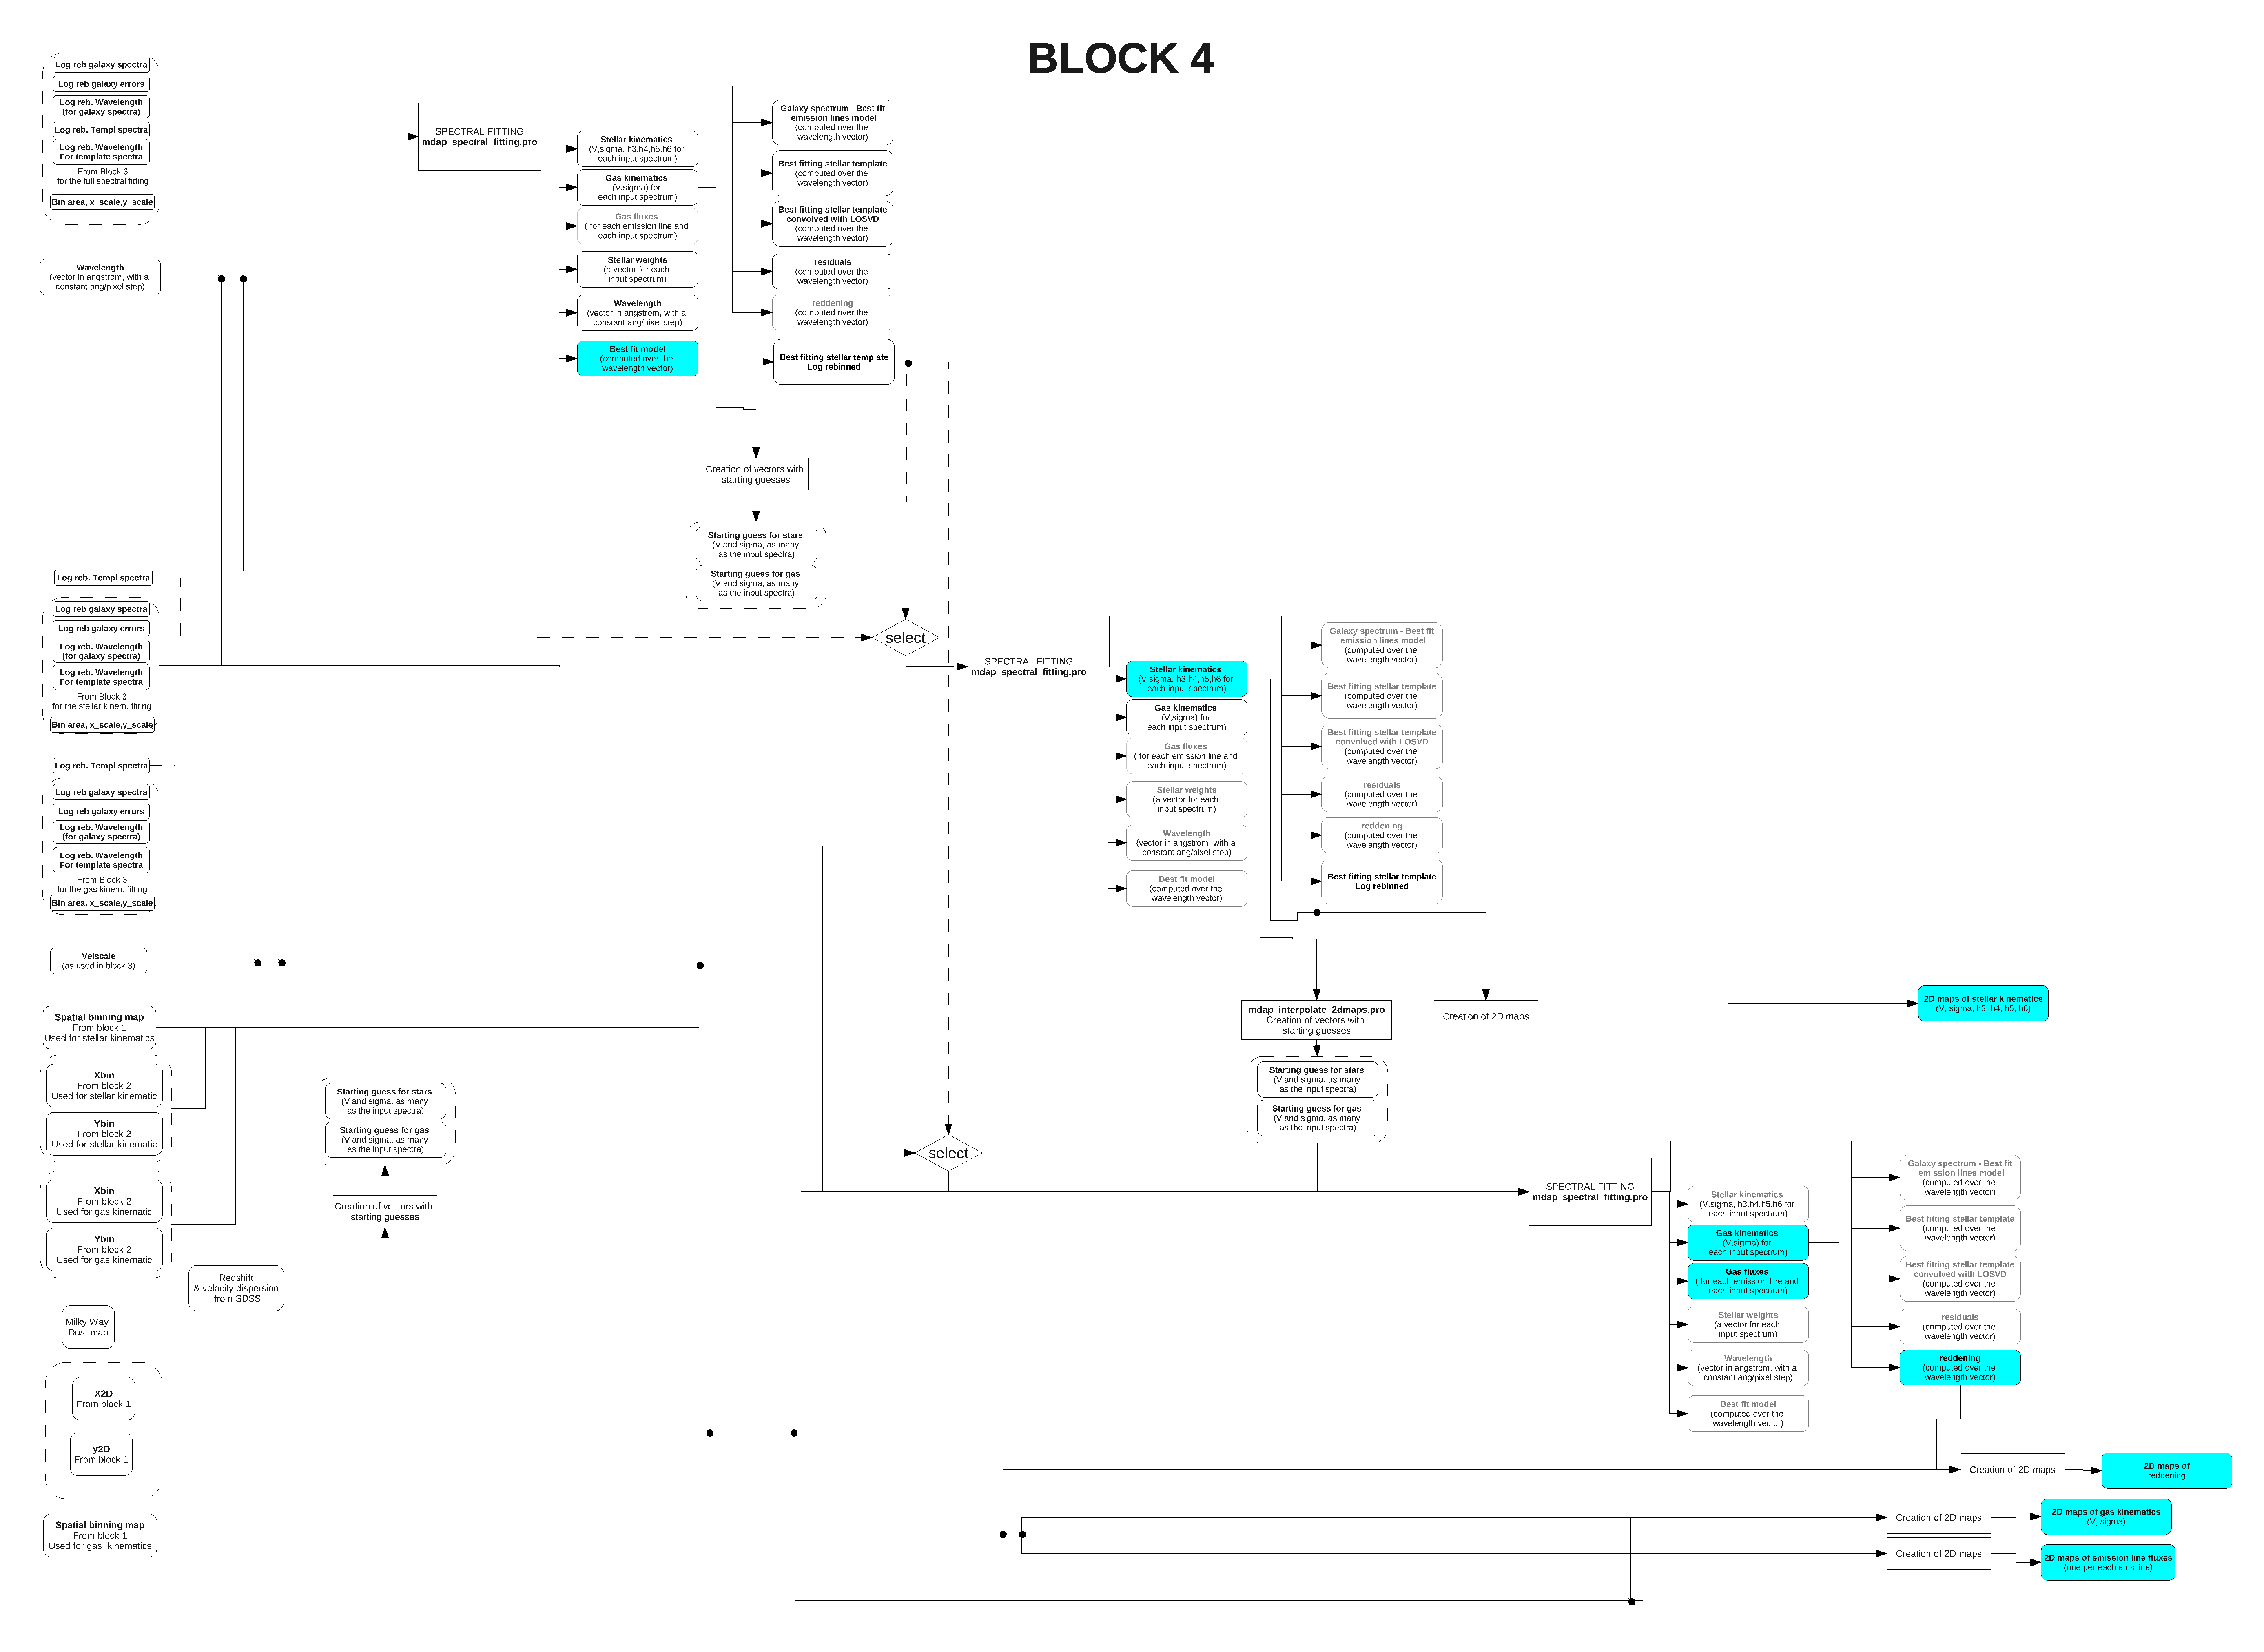
\psfig{file=figures/block4.ps, width=17cm, clip=, bb=35 25 560 620}
%\vspace*{0cm}
\caption{Workflow chart of the block 4 of the Data Analysis Pipeline.}
 \label{dap_fig:block4}
\end{center}
\end{figure}

\subsection{{\tt mdap\_create\_starting\_guesses.pro}}
\label{dap_sec:mdap_create_starting_guesses}


This interface is responsible to transform the kinematics measured on
a spatial binning scheme into starting guesses for the fit of another
spatial binning scheme. The main module that performs the computation
is mdap\_interpolate\_2dmaps.pro (see Section
\ref{dap_sec:mdap_interpolate_2dmaps}). 

Table \ref{dap_tab:mdap_create_starting_guesses} lists the inputs and
outputs of mdap\_create\_starting\_guesses.pro.


\begin{center}
\begin{longtable}{p{2.7cm}| p{11.1cm}}
\caption{Inputs and outputs  parameters of mdap\_create\_starting\_guesses.pro} \label{dap_tab:mdap_create_starting_guesses} \\
\hline
{\bf  INPUTS} & \\
\hline
\endfirsthead
\hline
\endhead
\hline
\endlastfoot
\hline
 input\_map  & Nx4 (or Nx2)  elements array containing the measurements  of velocity, velocity dispersion 
              of the N spectra to be used to get the starting guesses. If the keyword /h3h4 is set, input\_map
              must be Nx4 elements array, and previous measurements of h3 and h4 must be given.

              \medskip

              \ \ \ input\_map[*,0]: previous velocity measurements

              \ \ \ input\_map[*,1]: previous velocity dispersion measurements

              \ \ \ input\_map[*,2]: (optional) previous H3 measurements

              \ \ \ input\_map[*,3]: (optional) previous H4 measurements\\
%
input\_xbin  &  N elements array. X coordinates of the center of the spatial bins where the measurements in input\_map refer to.  \\
%
input\_ybin  &  N elements array. Y coordinates of the center of the spatial bins where the measurements in input\_map refer to.  \\
%
x2d          &  N'xM' elements array. Two dimensional map of X coordinates of a regular grid mapping the full field of view.  \\
%
y2d          &   N'xM' elements array. Two dimensional map of Y coordinates of a regular grid mapping the full field of view.       \\
%
velocity\_initial\_guess   & Float. Guess for the velocity to be used in the case of previous measurements are NaN, or not defined.  \\
%
velocity\_dispersion\_initial\_guess & Float. Guess for the velocity to be used in the case of previous measurements are NaN, or not defined, 
                                    or outside a fiducial interval $21<\sigma<499$ km/sec.     \\
%
H3\_initial\_guess  &  Float. Guess for the velocity to be used in the case of previous measurements are NaN, or not defined, or outside a fiducial
                          interval $-0.399 < h3 < 0.399$.  \\
%
H4\_initial\_guess  &  Float. Guess for the velocity to be used in the case of previous measurements are NaN, or not defined, or outside a fiducial
                          interval $-0.399 < h4 < 0.399$.  \\ 
%
output\_xbin &  M elements array. X coordinates of the center of the spatial bins where the starting guesses are to be computed. \\
%
output\_ybin & M elements array. Y coordinates of the center of the spatial bins where the starting guesses are to be computed. \\
\hline
{\bf  KEYWORD} & \\
\hline
/h3h4    &   If set, the guesses of Gauss Hermite moments (h3, h4) will be computed (otherwise set to H3\_initial\_guess and
             H4\_initial\_guess) . The input input\_map must contain h3 and h4 measurements.     \\
\hline
{\bf  OUTPUTS} & \\
\hline
output\_start\_guess &   Mx4 elements array containing the interpolated velues of of velocity, velocity dispersion of the N spectra 
             to be used as starting guesses. If the keyword /h3h4 is set, it will be Mx4 elements array.

      \medskip

   \  \  \                output\_start\_guess[*,0]: velocity interpolated on the  output\_xbin, output\_ybin, grid to be used as starting guesses.

   \  \  \           output\_start\_guess[*,1]: velocity dispersion interpolated on the  output\_xbin, output\_ybin, grid to be used as starting guesses.

   \  \  \            output\_start\_guess[*,2]: (optional) H3 interpolated on the  output\_xbin, output\_ybin, grid to be used as starting guesses.

   \  \  \            output\_start\_guess[*,3]: (optional) H4 interpolated on the  output\_xbin, output\_ybin, grid to be used as starting guesses.\\

\hline
\end{longtable}
\end{center}


\subsection{{\tt mdap\_spectral\_fitting.pro}}
\label{dap_sec:mdap_spectral_fitting}

This module is responsable for i) arranging the inputs from previous
modules/blocks and feed them into the main module that perform the fit
(mdap\_gandalf\_wrap.pro, see Section
\ref{dap_sec:mdap_gandalf_wrap.pro}) , and ii) re-arrange the outputs
of the fits for further processing.

The list of input/output parameters of mdap\_spectral\_fitting.pro is
given in Table \ref{dap_tab:mdap_spectral_fitting}.



%\begin{table}
\begin{center}
\begin{longtable}{p{2.7cm}| p{11.1cm}}
\caption{Inputs and outputs parameters of mdap\_spectral\_fitting.pro} \label{dap_tab:mdap_spectral_fitting} \\
\hline
\endfirsthead

\hline
\endhead

\hline
\endlastfoot

%\begin{tabular}{p{2.7cm}| p{2.5cm} |p{9cm}}
\hline
{\bf  INPUTS} &  \\
\hline
 galaxy &     [MxN  array]. It contains the N galaxy spectra to fit, logarithmically 
              sampled (natural log). Units: 1e-17 erg/s/cm$^2$/Angstrom. Spectra are defined of the
              M elements array loglam\_gal (see below).\\
%
  noise &     [MxN  array]. It contains the N error vectors for the
              N galaxy spectra. Same units as galaxy. Error vectors are defined of the
              M elements array loglam\_gal (see below).\\
%
  loglam\_gal& [M array]. It contains the log wavelength values where
             galaxy and noise spectra are defined. The vector must have a constant 
             log(angstrom) sampling. \\
%
  templates & [MM x NN array].  It contains the NN stellar template
            spectra, logarithmically sampled at the same \kms/pixel as the
            galaxy spectra. Same units as galaxy, except an arbitrary
            multiplicative factor.\\
%
 loglam\_templates & [MM dblarray]. It contains the log wavelength values where
            templates are sampled. It must have a constant log(angstrom) sampling.  \\
%
 velscale & [float].  Defines the (uniform) sampling of the input spectra, in \kms/pixel.\\
%;
\hline
%
{\bf OPTIONAL INPUTS } &  \\
\hline
 extra\_inputs & [string array] It contains other inputs
               that might be used in the fitting procedure, such as
               the number of polinomyal degree. Variable will be
               initialized with the IDL execute command.

                    {\tt for i = 0, n\_elements(extra\_inputs)-1 do d = execute(extra\_inputs[i])}

               EXAMPLE:  

                {\tt extra\_inputs=['MOMENTS=2','DEGREE=-1','MDEGREE=3', 'BIAS=0.2', 
                'reddening=[0.1,0]', 'LAMBDA=exp(loglam\_gal)']}.

              Warning: The reddening (stars and/or gas) fit is
              optional, and it is performed by the Gandalf module. If
              the reddening fit is required, MDEGREE and DEGREE are
              used as the input value for the pPXF run, but
              automatically set to 0 and -1 respectively for the
              Gandalf execution. \\
%           
 star\_kin\_starting\_ guesses& [N x 4 fltarray]. The stellar kinematics starting guesses for V, 
                           $\sigma$, H3, and H4 for the N galaxy spectra to fit.
                           Default values are 0. for V, H3, and H4, and 50 km/sec for sigma. 
                           Starting guesses values are overrided by
                           the /use\_ previos\_ guesses keyword, if set.\\
%
 gas\_kin\_starting\_ guesses & [N x 2 fltarray]. The emission line kinematics starting guesses for V, 
                           $\sigma$, for the N galaxy spectra to fit.
                           Default values are 0 \kms\ for V, and 50 \kms\ for sigma. 
                           Starting guesses values are overrided by
                           the /use\_previos\_guesses keyword, if set.\\
%
emission\_line\_ file &[string]. It contains the name of the file with the information of the
                    emission lines to be fitted.
                    The format must be compatible with the module that performs the fit of the emission lines. 
                    If Gandalf or S-Gandalf are used, the input file must be an ascii file with the 
                    following 9 columns as in the following example (comments starts with ''\#''):
                      \medskip
 
                    {\tt 
                    \#  ID  CODE \  wav  \ action  line    Int	Vel     $\sigma$ mode

                    \#  \ \ \ \ \ \ \  \ \ [\AA]  \ \ f/i/m   dbl?

                    \#   0   HeII\ \ 3203.15  \   m \ \ \ l   \  \ 1.0	\   0 \	10 	t25

                    \#   1   NeV  3345.81 \    m  \ \ \ l    \ \ 1.0  \   0 \   10      t25

                    \ \  2   NeV  3425.81  \   m  \ \ \ l   \ \ 1.0   \  0  \  10      t25

                    \ \  3   OII  3726.03   \ m  \ \ \ l   \ \  1.0 \	   0 \	10 	t25 }

                     \medskip

                     \begin{itemize}
                       \item {\tt ID} Unique integer identifyer of the emission line.

                       \item {\tt CODE}. String. Name of the element. Special characters as ``[``, ``.'' are not permitted.

                       \item {\tt wav}. Float. Rest frame wavelength of the emission line to fit. Warning, the
                         name of the emission line in the final DAP output will be defined by the string {\tt CODE} +''\_''+ {\tt ROUND(wav)}.

                         \item {\tt action}. String. Possible values are ``f'' (fit), ``m'' (mask), and ``i''
                           (ignore). All lines are masked in the pPXF run, and then fit in the Gandalf run,
                           unless they are marked with ``i'', in this latter case they will be ignored.

                        \item {\tt line}. String Possible values are ``l'' (line) or ``dN'' (doublet). In this
                          case, N indicates the line ID to which the  doublet is linked, linked to the line with
                          ID=N. For example, if emission line with {\tt ID=4} has {\tt line=''d3''}, then the 
                          emission line with {\tt ID=3} must have {\tt line = ``l''}.

                        \item {\tt int}. Float. Relative intensity of the gas emission (positive) or absorption 
                               (negative) lines. It is set to 1 for lines ({\tt line = ``l''}). For doublets, ( {\tt line = ``dN''}) 
                               it indicates the ration elements of the doublets.
                        \item {\tt vel}. Float. Guess of the velocity offset with respect the galaxy systemic velocity (ignored in the DAP)
                        \item {\tt sigma}. Float. Guess of the Velocity dispersion (ignored in the DAP)
                        \item {\tt mode}. String. Possible values are ``f'' (fit) or ``tN'' (tied). If a line has {\tt mode = tN}, its kinematics is tied 
                                          to the line with {\tt ID=N}. In this case, the line with {\tt ID=N} must have {\tt mode = f}.
                         \end{itemize} \\
%
 range\_v\_star  &[2 elements array]. It specifies the boundaries for the stellar best fit velocity (in \kms). Default: starting\_guess $\pm$ 2000 \kms.\\
%;
 range\_s\_star  &[2 elements array]. It specifies the boundaries for the stellar best fit velocity dispersion (in \kms). Default: $21 < \sigma < 499$ \kms.\\
%;
 range\_v\_gas   &[2 elements array]. It specifies the boundaries for the emission line best fit velocity (in \kms) Default: starting\_guess $\pm$ 2000 \kms.\\
%;
 range\_s\_gas &[2 elements array]. It specifies the boundaries for the
             emission line best fit velocity dispersion (in \kms). Default:
             starting\_guess $\pm$ 2000\kms.\\
%; 
wavelength\_input & [QQ elements array]. If specified, it will be
             used to create wavelength\_output (in \AA), i.e. the
             wavelength vector to interpolate the final results on. if
             keyword /rest\_frame\_log is set, the vector is set to
             exp(loglam\_templates), and user inpiut will be
             overwritten. In this case QQ = MM.  Suggested
             entry: use the exp(loglam\_templates). \\
%
external\_library & String that specifies the path to the external {\tt FORTRAN} library, which contains the fortran versions of mdap\_bvls.pro. 
                  If not specified, or if the path is invalid, the default internal IDL mdap\_bvls code is used. \\
%
mask\_range  & If defined, it specifies the wavelength ranges to mask in the fit. It must contain an even number of entries, in
           angstrom. E.g. mask\_range=[$\lambda_0$, $\lambda_1$, $\lambda_2$, $\lambda_3$, ....$\lambda_{(2n-1)}$, $\lambda_{(2n)}$] will mask all the pixels where the 
             $\lambda_0 < exp({\rm loglam\_gal}) <\lambda_1$; $\lambda_2 < exp({\rm loglam\_gal}) <\lambda_3$;  $\lambda_{(2n-1)} < exp({\rm loglam\_gal}) <\lambda_{(2n)}$.\\
%
fwhm\_instr\_ kmsec\_matrix & 2xW elements vector. It defines the instrumental FWHM as function of wavelength. 
                               fwhm\_instr\_ kmsec\_matrix[0,*] specifies the wavelength (in angstrom, at which the instrumental FWHM is measured. 
                               fwhm\_instr\_ kmsec\_matrix[1,*] specifies values of the instrumental FWHM (in km/sec) measured at fwhm\_instr\_ kmsec\_matrix[0,*]. 
                               If undefined, a constant instrumental FWHM=122.45 km/sec is adopted. \\
\hline 
 {\bf OPTIONAL KEYWORDS}  &  \\
\hline
%;
 /use\_previos\_ guesses &  If set, the starting guesses for spectrum $i-$th
                       will be the best fit values from spectrum
                      $(i-1)-$th (i$>0$). Input starting guesses will be ignored.\\
%;
 /fix\_star\_kin  &        If set, the stellar kinematics are not
                       fitted. The return values is that of the starting guesses. \\
%
 /fix\_gas\_kin   &        If set, the emission-lines kinematics are not fitted. The return values is that of the starting guesses. \\
%
/quiet     &            If set, some information are not printed on screen.\\
%
/rest\_ frame\_log & If set, the output spectra (galaxy\_minus\_ ems\_fit\_model, best\_fit\_model, residuals, 
             best\_template, and best\_template\_LOSVD\_conv) are produced at rest-frame wavelength.\\
%%
\hline
%
 {\bf OUTPUTS} &  \\
\hline
%;
  stellar\_ kinematics   &  [N x 5 flt array].  It contains the best fit values of V, $\sigma$, h3, h4, and $\chi^2$/DOF for each of the N fitted input galaxy spectra. If /fix\_star\_kin is set, the array is not defined.\\
%;
  stellar\_ kinematics\_err &[N x 5 flt arrary].  It contains the errors to the best fit values of V, $\sigma$, h3, h4, and $\chi^2$/DOF for each of the N fitted input galaxy spectra.\\
%;
  stellar\_weights        &[N x NN dbl array]. It contains the weights of the NN templates for each of the N input galaxy spectra.\\
%;
  emission\_line\_ kinematics &[N x 2 flt array].  It contains the best fit values of V, $\sigma$ (emission lines) for each of the N fitted
                            input galaxy spectra. If /fix\_gas\_kin is set, the array is not defined.\\
%;
 emission\_line\_ kinematics\_err & [N x 2 flt array].  It contains the errors to the best fit values of V, $\sigma$ (emission lines) for each of the N fitted input galaxy spectra. If /fix\_gas\_kin is set, the array is not defined.\\
%;
 emission\_line\_ intens  &[N x T flt array].  It contains the intensities of the T fitted emission lines for each of the N input galaxy spectra. Values are corrected for reddening.\\
%
 emission\_line\_ intens\_err &  [N x T flt array].  Errors associated to emission\_line\_intens \\
%
 emission\_line\_ equivW      & [N x T flt array]. It contains the Equivalent widths of the T fitted emission lines for each of the N input galaxy spectra.                            Equivalent widths are computed by the ratio of emission\_line\_fluxes and the median value of the stellar spectrum within 5 and 10 $\sigma$ from the emission line. $\sigma$ is the emission line velocity dispersion. \\
%
 emission\_line\_ fluxes\_err &  [N x T flt array].  Errors associated to emission\_line\_fluxes \\
%
 emission\_line\_ equivW      & [N x T flt array]. It contains the Equivalent widths of the T fitted emission lines for each of the N input galaxy spectra.                            Equivalent widths are computed by the ratio of emission\_line\_fluxes and the median value of the stellar spectrum within 5 and 10 $\sigma$ from the emission line. $\sigma$ is the emission line velocity dispersion. \\
%
 emission\_line\_ equivW\_err  & [N x T flt array]. Errors associated to emission\_line\_equivW  . \\
%
 wavelength\_ output     & [QQ elements flt array]. It will contain the wavelength values over which the output spectra are sampled (in \AA). 
                        Default: it is set to wavelength\_input (if defined), or automatically computed with the smallest lambda/pixel step obtained from exp(loglam\_gal). 
                        It is set to exp(LOGLAM\_TEMPLATES) if the keyword /rest\_ frame\_log is set.\\
%
 best\_fit\_model      &[N x QQ flt array]. It will contain the best fit models for each of the input galaxy spectra (dereddended if 
                       MW\_extinction is not zero), sampled over wavelength\_output. It is in rest-frame if the keyword /rest\_frame\_log is set. \\
%
 galaxy\_minus\_ ems\_fit\_model &[N x QQ flt array]. It will contain the input galaxy spectra minus the emission lines best fit models (dereddended if MW\_extinction is not zero), 
                      sampled over wavelength\_output, for each of the N input spectra. It is in rest-frame if the keyword /rest\_frame\_log is set\\
%
 best\_template &[N x QQ flt array]. It will contain the best fitting template for each of the N input galaxy spectra sampled over wavelength\_output (rest frame wavelength). \\
%
 best\_template\_ LOSVD\_conv &[N x QQ flt array]. It will contain the best fitting template for each of the N input galaxy spectra convolved by best fitting 
LOSVD and sampled over wavelength\_output (rest frame wavelength).\\
%
reddening\_ output &[N x 2 elements array]. Best fit values for the reddening of stars (reddening\_ output[*,0]) and gas (reddening\_ output[*,1]) for all the N galaxy spectra. 
                                             If the reddening fit is not requred, the output value is set to 0. (reddening\_output[*,0:1] = [0,0]). 
                                             If only the reddening of the stars is fitted, the reddening of the gas is set to 0 (reddening\_output[*,1] = 0).\\
%
reddening\_ output\_err &[N x 2 elements array]. Errors associated to reddening\_ output. If not fitted, the error is automatically set to 99.\\
% 
 residuals &[N x QQ flt array]. It contains the difference between the observed galaxy spectra and the best\_fit\_model, 
                            sampled over wavelength\_output. It is in rest-frame if the keyword /rest\_frame\_log is set\\
%
\hline
{\bf  OPTIONAL OUTPUTS} &  \\
version & string specifying the module version. If requested, the module is not execute and only version flag is returned.\\
\hline
\hline
\end{longtable}
\end{center}


%\begin{figure}
%\begin{center}
%%\hspace{-2cm}
%%\includegraphics[width=6cm,angle=90]{dap_workflow_1.ps}
%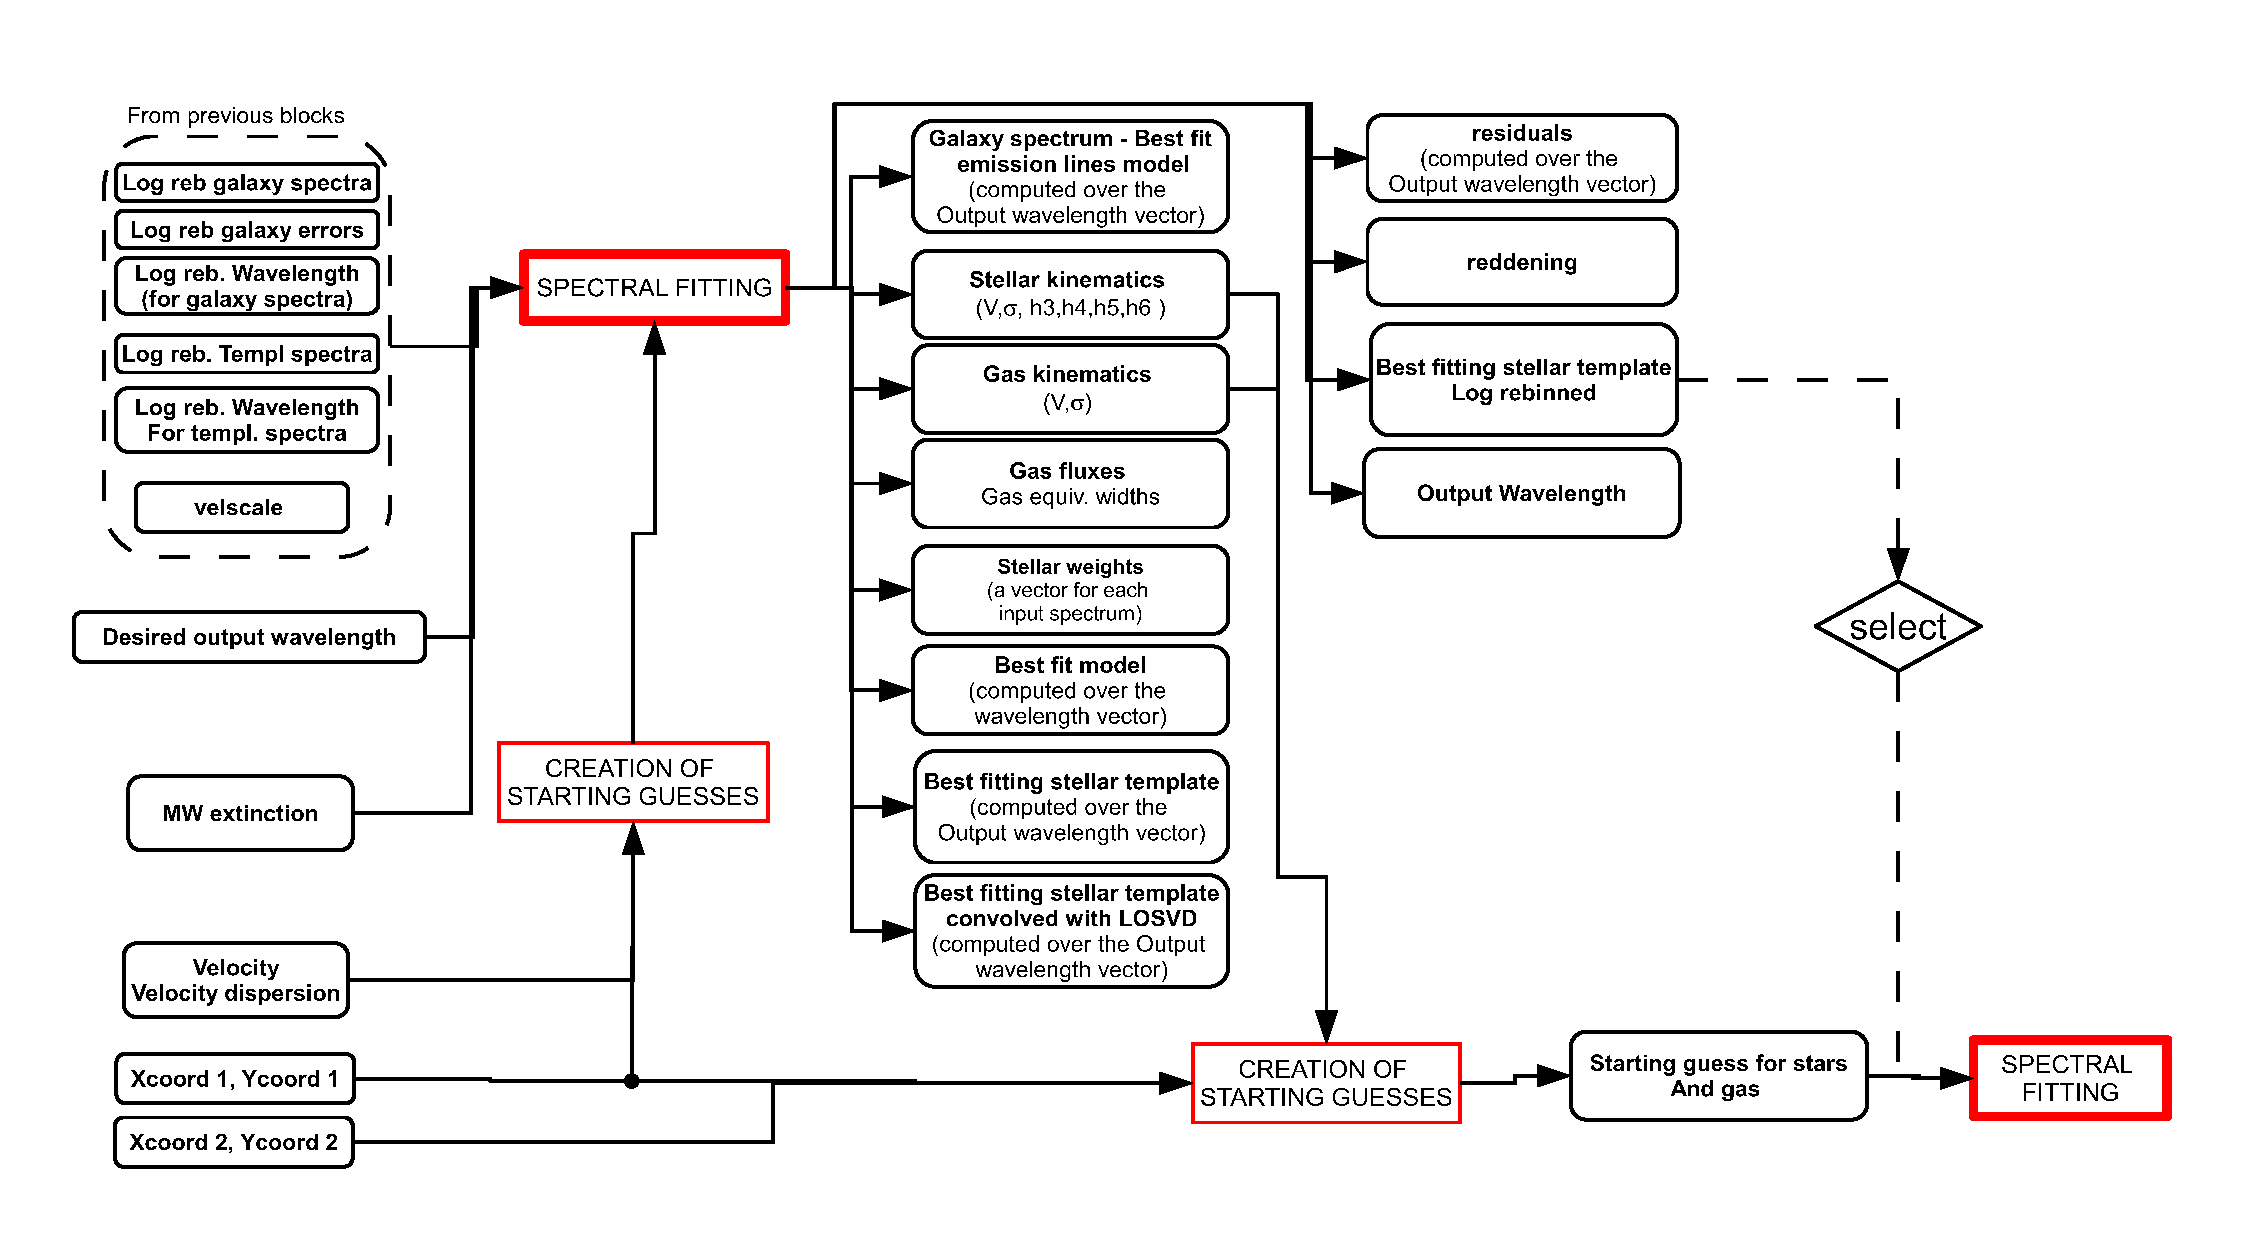
\psfig{file=figures/Block_4_zoom.ps, width=16cm, clip=}
%%\vspace*{0cm}
%\caption{Workflow chart of the block 4 of the Data Analysis Pipeline,
 % zoom around the first fit section.}
% \label{dap_fig:block4a}
%\end{center}
%\end{figure}


\section{DAP Block 5: Measurement of absorption line indices}
\label{dap_sec:block5}

This block is responsible for measuring the equivalent width of
absorption line indices on the galaxy spectra where the best fit model
for emission lines has been removed.

It requires the following inputs:
\begin{itemize}
 
\item The galaxy spectra with emission lines removed (from block 4).

\item The stellar velocity.

  \item The LSF as function of wavelenght (to a proper
broadening of the input spectra to the reference calibration system,
e.g. Lick, MILES).

\item The best fitting stellar template and the best fitting stellar
  template convolved by the best fitting LOSVD, for intrinsic
  broadening correction (from block 4).

\end{itemize}

The interface module in block 5 is {\tt mdap\_measure\_indices.pro}
(Section \ref{dap_sec:mdap_measure_indices}). Figure
\ref{dap_fig:block5} illustrates the flowchart of this module.  Table
\ref{dap_tab:mdap_measure_indices} describes the inputs and outputs of
this interface. The actual measurements are performed by the main
module {\tt mdap\_do\_measure\_indices.pro} (Section
\ref{dap_sec:mdap_do_measure_indices}).


\begin{figure}
\begin{center}
%\hspace{-2cm}
%\includegraphics[width=6cm,angle=90]{dap_workflow_1.ps}
\psfig{file=figures/block5.ps, width=16.5cm, clip=,bb= 22 363 566 816}
%\vspace*{0cm}
\caption{Workflow chart of mdap\_measure\_indices.pro, the interface
  module in block 5 of the Data Analysis Pipeline.}
 \label{dap_fig:block5}
\end{center}
\end{figure}


\subsection{{\tt mdap\_measure\_indices.pro}}
\label{dap_sec:mdap_measure_indices}

This interface is responsible for measuring the strength of the
absoprtion line indices, their errors, and correct them for galaxy
intrinsic broadening. Broadening correction is applied to the input
galaxy spectra to match the spectral resolution of the spectral
indices system (e.g. Lick). Input galaxy spectra must have emission
lines removed.

The measurement of the index is performed by the main module
mdap\_do\_measure\_indices.pro, see Section
\ref{dap_sec:mdap_do_measure_indices}.

Warning: ``D4000'' and ``TiO0p89'' (i.e. TiO0.89) indices are defined
as the ratio of the flux in the red and blue pseudocontinua. This
alternative configuration is hardwired in the
mdap\_measure\_indices.pro interface, and it is triggered by the index
name (i.e. be sure that the user input file with indices definitions
have these two names correcty spelled).

Broadening correction is done according to the following formula

\[
I_{\rm corr} = I_{\rm gal} \frac{I_{\rm templ}}{I_{\rm templ\ LOSVD}}
\]
for atomic indices, and 
\[
I_{\rm corr} = I_{\rm gal} + I_{\rm templ} - I_{\rm templ\ LOSVD}
\]
for molecular indices.  $I_{\rm corr}$ is the index line strength
corrected for intrinsic broadening, $I_{\rm templ}$ is the index line
strength measured on the best fitting stellar template, and $I_{\rm
  templ\ LOSVD}$ is the index line strength measured on the best
fitting stellar template convolved by the best fitting LOSVD.

The Convolution the input spectra to match a desired system is done by
the utility module mdap\_convol\_sigma (Section
\ref{dap_sec:mdap_convol_sigma}).

The list of input/output parameters for this module is given in Table
\ref{dap_tab:mdap_measure_indices}.


\begin{center}
\begin{longtable}{p{2.7cm}| p{11.1cm}}
\caption{Inputs and outputs parameters of mdap\_measure\_indices.pro} \label{dap_tab:mdap_measure_indices} \\
\hline
\endfirsthead
\hline
\endhead
\hline
\endlastfoot
\hline
{\bf  INPUTS} & \\
\hline
wavelength & [N elements array]. Vector containing the wavelenghts of the input spectra. The dispersion can be also not constant.\\
%
spectra & [T x N elements array].  Vector containing the T input galaxy spextra, with emission line removed. Spectra are defined over the vector wavelength.\\
%
best\_template & [T x N elements array]. Vector containing the T best fitting stellar templates obtained when fitting the kinematics of the input spectra. 
                Spectra are defined over the vector wavelength.\\
%
best\_template\_ LOSVD, & [T x N elements array]. Vector containing the T best fitting stellar templates, convolved with the best-fitting stellar LOSVD, obtained when 
                  fitting the kinematics of the input spectra. Spectra are defined over the vector wavelength. \\
%
stellar\_velocity & [T elements array]. Vector containing the best fitting stellar velocity for the T input spectra in km/sec. P.S. Set it to zero if the input spectra are in rest-frame\\
%
residuals & [T x N elements array]. Vector containing the residuals from the best fit model to the input galaxy spectra. Residuals are defined over the vector wavelength.  \\
%
fwhm\_diff\_ indices\_ & [N elements array]. Vector that specifies the FWHM($\lambda$) (in \AA) that should be used to broaden the spectra, best\_template, and best\_template\_LOSVD to match the spectral resolution of the spectral indices system.\\
\hline 
{\bf OPTIONAL INPUTS} & \\
\hline
dir=dir  &  Directory where to store the ps files showing the measurements \\
%
\hline
{\bf OUTPUTS} & \\
\hline
abs\_line\_ indices & [T x Nind array]. Absorption line indices of the T inut spectra, corrected for intrinsic broadening. The Nind measure indices are defined in 
   aborption\_line\_ indices\_definition, specified in the configuration file (see Section \ref{dap_sec:configuration}).\\
%
abs\_line\_ indices\_errors & [T x Nind array]. Errors associated to abs\_line\_ indices. \\
%
abs\_line\_ indices\_template &  Absorption line indices measured on best\_template \\
%
abs\_line\_ indices\_template\_ losvd &   Absorption line indices measured on best\_template\_ LOSVD.\\
\hline
{\bf  OPTIONAL OUTPUTS} &  \\
\hline
version & string specifying the module version. If requested, the module is not execute and only version flag is returned.\\
\hline
\hline
\end{longtable}
\end{center}



 

\section{DAP Block 6: Radial properties of high level data products}
\label{dap_sec:block6}

This block measures the radial properties of the absorption line
indices (part 1) and the kinematics i.e. rotation curves (parts 2 and
3).

The first part uses the restframed galaxy spectra (and errors) with
removed emission lines produced in block 4 from the third spatial
binning. Spectra are grouped according to elliptical bins (using the
user input mean ellipticity an position angle) and added
together. Then the spectra are fitted ({\tt mdap\_spectral\_fitting},
Section \ref{dap_sec:mdap_spectral_fitting}) and the indices are
measures ({\tt mdap\_measure\_indices.pro}, Section
\ref{dap_sec:mdap_measure_indices}).  In the spectral fitting,
emission lines are fitted again (except NaD absorptions), to remove
additional residuals; each emission line has can have its own velocity
and velocity dispersion. Stellar kinematics is bound to be within $-50
< V < 50$ km/sec. Reddening is not fitted.

Then, the output spectra (with residual emission lines removed, along
with the best fitting stellar template (to correct for intrinsic
broadening) are used to measure the absorption line indices.

The second part uses the stellar and emission line kinematics from
block 4 to measure the kinematic position angle, kinematic center,
kinematic axial ratio, rotation curve and amplitude of
inflows/outflows. The interface that handles the second part is {\tt
  mdap\_do\_kinemetry.pro} (Section \ref{dap_sec:mdap_do_kinemetry}),
which implements kinemetry.pro by Kraijnovic et al. 2008.

The third part uses the stellar two-dimensional kinematics to compute
the radial profile of the specific angular momentum ($\lambda(R)$),
the $V/\sigma(R)$, and $\sigma(R)$ (see Section
\ref{dap_sec:mdap_do_k_rprofiles}).


\subsection{mdap\_spatial\_radial\_binning.pro}
\label{dap_Sec:mdap_spatial_radial_binning}

T.B.D.


\subsection{{\tt mdap\_do\_kinemetry.pro}}
\label{dap_sec:mdap_do_kinemetry}

This interface module is responsible to pass the measured stellar and
emission line velocities to the kinemetry module, which measures the
rotation curves, outflows and inflows motions, mean kinematic position
angle, and mean kinematic axial ratio of stars and gas. The kinemetry
module uses the kinemetry.pro module by Kraijnovic et al. 2005
(Section \ref{dap_sec:mdap_kinemetry})

The following steps are executed:

 \begin{itemize}

  \item The galaxy image is used to determine the galaxy center. If
    the center is outside a $3''\times 3''$ box aroud the center of
    the field of view, the galaxy center is automatically set to
    (0,0), i.e. the center of the field of view. The galaxy kinematic
    center is set to be the galaxy photometric center in the
    kinemetry.pro runs.


 \item A first kinemetry run is executed, to get the The galaxy
   systemic velocity is kept constant at all radii (a first
   kinemetry.pro run is executed to measure the systemic velocities
   Vs$_i$at each i-th radius. The galaxy systemic velocity (Vsyst) and
   its 1sigma error (Vsyst\_std) are computed by the median and the
   standard deviation of the systemic velocities Vs$_i$).

 \item A second kinemetry run is executed, fixing the kinematic center
   and the systemic velocity. In this run, the kinematic position
   angles (PA$_i$) and flattening (q$_i$) are measured for each
   radius. The galaxy mean kinematic position angle (PA\_kin) and its
   error (PA\_kin\_std) are measured as the median and standard
   deviation of all the PA$_i$ previously measured.  The galaxy mean
   kinematic axial ratio (q\_kin) and its error (q\_kin\_std) are
   measured as the median and standard deviation of all the q$_i$
   previously measured.

\item A third and final kinemetry run is executed, fixing the
  kinematic center, position angle, and axial ratio determined in the
  previous runs. This last run determines the rotation velocity, and
  expansion velocity (i.e. inflows/outflows) for several radii.

\end{itemize}


Table \ref{dap_tab:mdap_do_kinemetry} lists the inputs and outputs of
the interface module mdap\_do\_kinemetry.pro.

\begin{center}
\begin{longtable}{p{2.7cm}| p{11.1cm}}
\caption{Inputs and outputs parameters of
  mdap\_do\_kinemetry.pro} \label{dap_tab:mdap_do_kinemetry}
\\ \hline \endfirsthead

\hline
\endhead

\hline
\endlastfoot

\hline 
{\bf INPUTS} & \\ 
\hline 

image & NxM array. Galaxy image. It is used to determine the location
        of the center.\\
%
x2d & NxM array. X coordinates corresponding to image (0,0 is the
     center of the field of view.\\
% 
y2d NxM array. Y coordinates corresponding to image (0,0 is the
     center of the field of view.\\
%
x & T elements array. X coordinates at which the velocites are measured. \\
%
y & T elements array. X coordinates at which the velocites are measured. \\
%
velocity & T elements array. The measured velocities (in km/sec).\\
%
velocity\_err & T elements array. The measured velocity errors (in km/sec).\\
%
\hline
{\bf OUTPUTS} & \\
\hline
PA\_kin &    Median kinematic position angle used to determine Vrot and Vexp (third kinemetry.pro run). \\ 
%
PA\_kin\_std & Standard deviation of the kinematic position angles measured in the second kinemetry run. \\
%
q\_kin &  Median kinematic axial ratio used to determine Vrot and Vexp (third kinemetry.pro run). \\ 
%
q\_kin\_std & Standard deviation of the kinematic axial ratio measured in the second kinemetry run. \ \\ 
%
Vsyst & Systemic velocity used to determine Vrot and Vexp (third kinemetry.pro run) \\ 
%
Vsyst\_std & tandard deviation of the systemic velocities determined in the first kinemetry run.\\ 
%
Rad\_kin & W elements array. Semi major axis of the ellipses where Vrot and Vexp are measured. \\ 
%
Vrot & W elements array. Rotational velocity measured at Rad\_kin. \\ 
%
Vrot\_err & W elements array. Errors on Vrot. \\ 
%
Vexp & W elements array. Outflow/Inflow velocity measured at Rad\_kin. \\ 
%
Vexp\_err & W elements array. Errors on Vexp. \\ 
%
gal\_center\_x & Float. X coordinate of the galaxy center (0,0 is the center of the field of view). \\  
%
gal\_center\_y & Float. Y coordinate of the galaxy center (0,0 is the center of the field of view).\\ 
\hline
{\bf OPTIONAL OUTPUTS}  & \\
\hline
 version  & String containin the module version. If requested, the module is not executed 
           and only version flag is returned.\\
\hline
\hline
\end{longtable}
\end{center}


\subsection{mdap\_do\_k\_rprofiles.pro}
\label{dap_sec:mdap_do_k_rprofiles}).

T.B.D.




\section{DAP Block 7: Stellar population analysis}
\label{dap_sec:block7}
T.B.D.

\section{DAP Block 8: Properties of the emission lines}
\label{dap_sec:block8}
T.B.D.

\section{DAP Block 9: Mass modeling}
\label{dap_sec:block9}
T.B.D.


\chapter{Main modules}
\label{dap_chap:dap_modules}

In this Chapter we describe the main modules of the DAP.

\section{{\tt mdap\_calculate\_spectrum\_sn.pro}}
\label{dap_sec:mdap_calculate_spectrum_sn}

bla bla bla


\section{{\tt mdap\_do\_log\_rebin.pro}}
\label{dap_sec:mdap_do_log_rebin}

This module is called by the mdap\_log\_rebin.pro interface and
performs the actual logarithmic resampling. It has been originally
written by M. Cappellari within the ppxf package. Here we report the
original description of the procedure written by M. Cappellari.

\medskip

 NAME: MDAP\_DO\_LOG\_REBIN

\medskip

 PURPOSE: Logarithmically rebin a spectrum, while rigorously
 conserving the flux (if the keyword $\backslash$flux is set).
 Basically the photons in the spectrum are simply ridistributed
 according to a new grid of pixels, with non-uniform size in the
 spectral direction.

 This routine makes the `standard' zero-order assumption that the
 spectrum is *constant* within each pixels. It is possible to perform
 log-rebinning by assuming the spectrum is represented by a piece-wise
 polynomial of higer degree, while still obtaining a uniquely defined
 linear problem, but this reduces to a deconvolution and amplifies
 noise.

 This same routine can be used to compute approximate errors of the
 log-rebinned spectrum. To do this type the command:
    \[
        {\rm MDAP\_DO\_LOG\_REBIN, lamRange, err}^2{\rm , err2New}
    \]
 and the desired errors will be given by SQRT(err2New).  NB: This
 rebinning of the error-spectrum is very *approximate* as it does not
 consider the correlation introduced by the rebinning!

The list of inputs/outputs of the mdap\_do\_log\_rebin.pro is given in
Table \ref{dap_tab:mdap_do_log_rebin}.

\begin{center}
\begin{longtable}{p{2.7cm}| p{11.1cm}}
\caption{Inputs and outputs parameters of mdap\_do\_log\_rebin.pro} \label{dap_tab:mdap_do_log_rebin} \\
\hline
\endfirsthead

\hline
\endhead

\hline
\endlastfoot

%\begin{tabular}{p{2.7cm}| p{2.5cm} |p{9cm}}
\hline
{\bf  INPUTS} &  \\
\hline
LAMRANGE & two elements vector containing the central wavelength
       of the first and last pixels in the spectrum, which is assumed
       to have constant wavelength scale! E.g. from the values in the
       standard FITS keywords: LAMRANGE = CRVAL1 + [0, CDELT1 * (NAXIS1-1)].
       It must be LAMRANGE[0] < LAMRANGE[1].\\
%
SPEC:& N elements array. The input spectrum. \\
%
\hline
{\bf  OUTPUTS} &  \\
\hline
SPECNEW & M elements array. The logarithmically rebinned spectrum. \\
%
 LOGLAM & log(lambda)M elements array. natural logarithm (ALOG) of the central 
       wavelength of each pixel. This is the log of the geometric 
       mean of the borders of each pixel.\\
%
\hline
{\bf  OPTIONAL KEYWORDS} &  \\
\hline
/FLUX: & Set this keyword to preserve total flux. In this case the 
       log rebinning changes the pixels flux in proportion to their 
       dLam so the following command will show large differences 
       beween the spectral shape before and after LOG\_REBIN:

       \medskip

        \ \   {\tt plot, exp(logLam), specNew}  

       \smallskip

        \ \   {\tt oplot, range(lamRange[0],lamRange[1],n\_elements(spec)), spec}

       \medskip

       By default, when this keyword is *not* set, the above two lines
       produce two spectra that almost perfectly overlap each
       other. Do not set /flux for MaNGA data.\\
%
OVERSAMPLE: & Oversampling can be done, not to loose spectral resolution, 
       especally for extended wavelength ranges and to avoid aliasing.
       Default: OVERSAMPLE=1, i.e. Same number of output pixels as input.\\
%
VELSCALE: &velocity scale in km/s per pixels. If this variable is
       not defined, then it will contain in output the velocity scale.
       If this variable is defined by the user it will be used
       to set the output number of pixels and wavelength scale.\\
\hline
\end{longtable}
\end{center}


\section{{\tt mdap\_voronoi\_2d\_binning.pro}}
\label{dap_sec:mdap_voronoi_2d_binning}

This procedure is taken from the Voronoi Binning procedure by
Cappellari \& Copin (2003).  It has been modified so it automatically
relaxes the minimal $S/N$ requirements to have at least 1 bin in the
field of view. Table \ref{dap_tab:mdap_voronoi_2d_binning} lists the
inputs and outputs required for this module.


\begin{center}
\begin{longtable}{p{2.7cm}| p{11.1cm}}
\caption{Inputs and outputs parameters of mdap\_voronoi\_2d\_binning} \label{dap_tab:mdap_voronoi_2d_binning} \\
\hline
\endfirsthead
\hline
\endhead
\hline
\endlastfoot
\hline
{\bf  INPUTS} &  \\
\hline
X &[flt array] Vector containing the X coordinate of the pixels to bin.
             Arbitrary units can be used (e.g. arcsec or pixels).
            In what follows the term ?pixel? refers to a given
            spatial element of the dataset (sometimes called ?spaxel? in
            the IFS community): it can be an actual pixel of a CCD
            image, or a spectrum position along the slit of a long-slit
            spectrograph or in the field of view of an IFS
            (e.g. a lenslet or a fiber).
            It is assumed here that pixels are arranged in a regular
            grid, so that the pixel size is a well defined quantity.
            The pixel grid however can contain holes (some pixels can be
            excluded from the binning) and can have an irregular boundary.
            See the above reference for an example and details.\\
%
Y  &[flt array]. Vector (same size as X) containing the Y coordinate
            of the pixels to bin.\\
%
SIGNAL  &[flt array]. Vector (same size as X) containing the signal
            associated with each pixel, having coordinates (X,Y).
            If the `pixels' are actually the apertures of an
            integral-field spectrograph, then the signal can be
            defined as the average flux in the spectral range under
            study, for each aperture.
            If pixels are the actual pixels of the CCD in a galaxy
            image, the signal will be simply the counts in each pixel.\\
%
NOISE  &[flt array]. Vector (same size as X) containing the corresponding
            noise (1 sigma error) associated with each pixel.\\
%
TARGETSN & [float]. The desired signal-to-noise ratio in the final
            2D-binned data. E.g. a S/N$\sim$50 per pixel may be a
            reasonable value to extract stellar kinematics
            information from galaxy spectra.\\
\hline
{\bf  INPUT KEYWORDS:}      &    \\
  /NO\_CVT&  Set this keyword to skip the Centroidal Voronoi Tessellation
           (CVT) step (vii) of the algorithm in Section 5.1 of
           Cappellari \& Copin (2003).
           This may be useful if the noise is strongly non Poissonian,
           the pixels are not optimally weighted, and the CVT step
           appears to introduces significant gradients in the S/N.
           A similar alternative consists of using the /WVT keyword below.\\
%
    /PLOT&   Set this keyword to produce a plot of the two-dimensional
           bins and of the corresponding S/N at the end of the
           computation.\\
%
   /QUIET&   by default the program shows the progress while accreting
           pixels and then while iterating the CVT. Set this keyword
           to avoid printing progess results.\\
%
     /WVT&   When this keyword is set, the routine bin2d\_cvt\_equal\_mass is
           modified as proposed by Diehl \& Statler (2006, MNRAS, 368, 497).
           In this case the final step of the algorithm, after the bin-accretion
           stage, is not a modified Centroidal Voronoi Tessellation, but it uses
           a Weighted Voronoi Tessellation.
           This may be useful if the noise is strongly non Poissonian,
           the pixels are not optimally weighted, and the CVT step
           appears to introduces significant gradients in the S/N.
           A similar alternative consists of using the /NO\_CVT keyword above.
           If you use the /WVT keyword you should also include a reference to
           `the WVT modification proposed by Diehl \& Statler (2006).'\\
%
\hline
{\bf  OUTPOUTS:}        &    \\
   BINNUMBER &[flt array]. Vector (same size as X) containing the bin number assigned
           to each input pixel. The index goes from zero to Nbins-1.
           This vector alone is enough to make *any* subsequent
           computation on the binned data. Everything else is optional!\\
%
     XBIN &[flt array].  Vector (size Nbins) of the X coordinates of the bin generators.
           These generators uniquely define the Voronoi tessellation.\\
%
     YBIN &[flt array].  Vector (size Nbins) of Y coordinates of the bin generators.\\
%
     XBAR &[flt array].  Vector (size Nbins) of X coordinates of the bins luminosity
           weighted centroids. Useful for plotting interpolated data.\\
%
     YBAR &[flt array].  Vector (size Nbins) of Y coordinates of the bins luminosity
           weighted centroids.\\
%
       SN &[flt array].  Vector (size Nbins) with the final SN of each bin.\\
%
  NPIXELS &[flt array].  Vector (size Nbins) with the number of pixels of each bin.\\
%
    SCALE &[flt array].  Vector (size Nbins) with the scale length of the Weighted
           Voronoi Tessellation, when the /WVT keyword is set.
           In that case SCALE is *needed* together with the coordinates
           XBIN and YBIN of the generators, to compute the tessellation
           (but one can also simply use the BINNUMBER vector).\\
\hline
\end{longtable}
\end{center}



\section{{\tt mdap\_gandalf\_wrap.pro}}
\label{dap_sec:mdap_gandalf_wrap}

This main module fits an input galaxy spectrum with a series of stellar
templates and gas emission lines to derive the stellar and emission
lines kinematics, and the fluxes and equivalent width of the emission
lines.

The fit of the stellar kinematics is done using an implementation of
the pPXF routine (Cappellari \& Emsellem 2004, see Section
\ref{dap_sec:mdap_ppxf}), the fit of the emission line kinematics, the
weights of the stellar templates, (and reddening, if reuired) is done
using an implementation of the Gandalf routine (Sarzi et al. 2006, see
Section \ref{dap_sec:mdap_gandalf}).

The reddening of stars and gas (Balmer decrement) are fitted, if
required, using the Calzetti extinction law ( Calzetti et al. 2000,
see Section \ref{dap_sec:mdap_dust_calzetti}).

The steps performed by the {\tt mdap\_gandalf\_wrap.pro} main module
are:


\begin{itemize}

\item selection of regions to mask. These are:
   \begin{itemize} 

      \item the regions around emission lines; their location is
        computed using the velocity initial guess, and the width of
        the region to mask is set to 250 km/sec.

      \item The regions defined by the mask\_range input keyword, if
        provided.

   \end{itemize}

\item Run pPXF to measure the stellar kinematics. Additive and
  multiplicative polynomials are used in the fit, if specified in the
  user in the configuration file. The fit of the reddening is not
  performed. Note: The stellar kinematics is free to vary within the
  boundaries specified by the user (keywords range\_v\_star and
  range\_s\_star). This is an implementation to the original pPPXF
  procedure by Cappellari \& Emsellem (2004).

\item Remove the masks around the emission lines, but keeping the
  masks defined by the mask\_range input keyword (if defined).

\item Run Gandalf to measure the gas emission lines kinematics, and
  intensities. Additive polynomials are not used. Multiplicative
  polynomials are used (as in the previous pPXF run) only if the
  reddening is not fitted, otherwhise they are set to 0. Note: The gas
  kinematics is free to vary within the boundaries specified by the
  user (keywords range\_v\_gas and range\_s\_gas).  Also, the
  instrumental dispersion of the gas is assumed to vary with
  wavelength, therefore each emission line has its own value for the
  instrumental dispersion.  These are two implementations to the
  original Gandalf procedure by Sarzi et al. (2006).

\item Compute gas fluxes and equivalent widths (values are corrected
  for reddening, if reddening fit is required) from the emission line
  intensities.

\item Computation of the mean kinematics of the emission lines. The
  mean gas velocity and velocity dispersions are defined as the flux
  weighted average of the velocities and velocity dispersions of the
  detected individual emission lines.


\end{itemize}

Table \ref{dap_tab:mdap_gandalf_wrap} lists the inputs and outputs
parameters of the mdap\_gandalf\_wrap.pro module.


\begin{center}
\begin{longtable}{p{2.7cm}| p{11.1cm}}
\caption{Inputs and outputs parameters of
  mdap\_gandalf\_wrap.pro} \label{dap_tab:mdap_gandalf_wrap}
\\ \hline \endfirsthead

\hline
\endhead

\hline
\endlastfoot

%\begin{tabular}{p{2.7cm}| p{2.5cm} |p{9cm}}
\hline
{\bf  INPUTS} &  \\
\hline
templates & [MM x NN array].  It contains the NN stellar template
            spectra, logarithmically sampled at the same \kms/pixel as the
            galaxy spectra. Same units as galaxy, except an arbitrary
            multiplicative factor.\\
%
loglam\_templates & [MM dblarray]. It contains the log wavelength values where
            templates are sampled. It must have a constant log(angstrom) sampling.  \\
%
galaxy & [N elements array]. Galaxy spectrum, logarithically rebinned, to be fitted. \\
%
loglam\_gal & [N elements array]. $log(\lambda)$ values where the galaxy spectrum is defined. \\
%
noise & [N elements array]. Error vector associated to galaxy, defined over the loglam\_gal vector. \\
%
velscale & [float].  Defines the (uniform) sampling of the input spectra, in \kms/pixel.\\
% 
start\_ & 6 elements array containing the starting guesses:
            \ \ start\_[0] stellar veocity (km/sec)

            \ \ start\_[1] stellar velocity dispersion (km/sec)

             \ \ start\_[2] stellar h3 Gauss Hermite moment

            \ \ start\_[3] stellar h4 Gauss Hermite moment

            \ \ start\_[4] gas velocity (km/sec)

            \ \ start\_[5] gas velocity dispersion (km/sec). \\
%
\hline
{\bf  OPTIONAL INPUTS} &  \\
\hline
EMISSION\_ SETUP\_FILE & As in Table \ref{dap_tab:mdap_spectral_fitting}. \\
%
BIAS & As used Table  \ref{dap_tab:mdap_ppf}. \\
%
MDEGREE & Integer. Degree of multiplicative polynomials to be used in the pPXF fit and in the Gandalf fit (if reddening is not fitted). 
           Default: 0 (no multiplicative polynomials are used).\\
%
DEGREE &  Integer. Degree of multiplicative polynomials to be used in the pPXF only. 
           Default: -1 (no additive polynomials are used).\\
% 
reddening &  1 or 2 elements array. If specified in input, it triggers the
             fittind of the stellar reddening (1 element array) and the gas
             reddening (balmer decrement) (2 elements array). 
             In output it will contain the best fit reddening values. \\
%
 range\_v\_star  &[2 elements array]. It specifies the boundaries for the stellar best fit velocity (in \kms). Default: starting\_guess $\pm$ 2000 \kms.\\
%;
 range\_s\_star  &[2 elements array]. It specifies the boundaries for the stellar best fit velocity dispersion (in \kms). Default: $21 < \sigma < 499$ \kms.\\
%;
 range\_v\_gas   &[2 elements array]. It specifies the boundaries for the emission line best fit velocity (in \kms) Default: starting\_guess $\pm$ 2000 \kms.\\
%;
 range\_s\_gas &[2 elements array]. It specifies the boundaries for the
             emission line best fit velocity dispersion (in \kms). Default:
             starting\_guess $\pm$ 2000\kms.\\
%
mask\_range  & If defined, it specifies the wavelength ranges to mask in the fit. It must contain an even number of entries, in
           angstrom. E.g. mask\_range=[$\lambda_0$, $\lambda_1$, $\lambda_2$, $\lambda_3$, ....$\lambda_{(2n-1)}$, $\lambda_{(2n)}$] 
            will mask all the pixels where the 
             $\lambda_0 < exp({\rm loglam\_gal}) <\lambda_1$; $\lambda_2 < exp({\rm loglam\_gal}) <\lambda_3$; 
             $\lambda_{(2n-1)} < exp({\rm loglam\_gal}) <\lambda_{(2n)}$.\\
%
external\_library & String that specifies the path to the external {\tt FORTRAN} library, which contains the fortran versions of mdap\_bvls.pro. 
                  If not specified, or if the path is invalid, the default internal IDL mdap\_bvls code is used. \\
% 
INT\_DISP    &N elements array, containing the instrumental velocity dispersion (in km/sec) for all the N emission lines
               measured at their observed wavelengths (defined by the gas starting velocity guess). \\
\hline
{\bf KEYWORDS}  & \\
/FOR\_ERRORS    & If specified, it will trigger the computation of the emission lines error
                  (see Section \ref{dap_sec:mdap_gandalf}). Mandatory for the DAP workflow.\\
%
/fix\_star\_ kin & If set, the stellar kinematics will be fixed to the starting guesses values.\\
%
/fix\_gas\_ kin & If set, the gas kinematics will be fixed to the starting guesses values.\\
%
\hline
{\bf  OUTPUTS} &  \\
\hline
sol &  9 elements array containing the best fit kinematic parameters. 

       \ \ sol[0]:stellar velocity (km/sec).

       \ \ sol[1]:stellar velocity dispersion  (km/sec).

       \ \ sol[2]:stellar h3 Gauss-Hermite moment.

       \ \ sol[3]:stellar h4 Gauss-Hermite moment.

       \ \ sol[4]:stellar h5 Gauss-Hermite moment (not used).

       \ \ sol[5]:stellar h6 Gauss-Hermite moment (not used).

       \ \ sol[6]:$\chi^2$.

       \ \ sol[7]: mean flux weighted velocity of the emission lines (km/sec).

       \ \ sol[8]: mean flux weighted velocity dispersion (km/sec).  \\
%
gas\_intens &  N elements array, where N is the number of emission lines defined in EMISSION\_ SETUP\_FILE, 
                 whithin the wavelength range loglam\_gal. It specifies the intensity (corrected for reddening) 
                 of the emission lines. The intensities of lines in a multiplet are constrained by the flux ratio 
                 defined in the EMISSION\_ SETUP\_FILE (see Table \ref{dap_tab:mdap_spectral_fitting}). \\
%
gas\_fluxes & N elements array, where N is the number of emission lines defined in EMISSION\_ SETUP\_FILE, 
                 whithin the wavelength range loglam\_gal. It specifies the fluxes  (corrected for reddening) 
                 of the emission lines. The intensities of lines in a multiplet are constrained by the flux ratio 
                 defined in the EMISSION\_ SETUP\_FILE (see Table \ref{dap_tab:mdap_spectral_fitting}). \\
%
gas\_ew & N elements array, where N is the number of emission lines defined in EMISSION\_ SETUP\_FILE, 
                 whithin the wavelength range loglam\_gal. It specifies the equivalent widhts (corrected for reddening) 
                 of the emission lines. The intensities of lines in a multiplet are constrained by the flux ratio 
                 defined in the EMISSION\_ SETUP\_FILE (see Table \ref{dap_tab:mdap_spectral_fitting}). Equivalent widths 
                 are computed by comparing the emission line flux with the median flux of the stellar 
                 continuum in the spectral region  $\lambda_{i} - 10 \cdot FWHM_i < \lambda < \lambda_{i} - 5 \cdot FWHM_i $ and 
                 $\lambda_{i} +5 \cdot FWHM_i < \lambda < \lambda_{i} +10 \cdot FWHM_i $, where $\lambda_{i}$ is the central wavelength 
                  of the i-th emission line, and FWHM\_i is its measured FWHM (intrinsic plus instrumental). \\
%
gas\_intens\_err  & N elements array, error on gas\_intens. \\ 
%
gas\_fluxes\_err  & N elements array, error on gas\_fluxes. \\
%
gas\_ew\_err &N elements array, error on gas\_ew. \\
%
\hline
{\bf  OPTIONAL OUTPUTS} &  \\
\hline
bestfit   &   N elements array containing the best fit model (stars + gas), defined over the loglam\_gal vector. \\.
%
ERROR   & 8 elements array, containing the errors on the kinematic parameters.
       \ \ ERROR [0]: error on the stellar velocity (km/sec).

       \ \ ERROR [1]: error on the stellar velocity dispersion  (km/sec).

       \ \ ERROR [2]: error on the stellar h3 Gauss-Hermite moment.

       \ \ ERROR [3]: error on the stellar h4 Gauss-Hermite moment.

       \ \ ERROR [4]: error on the stellar h5 Gauss-Hermite moment (not used).

       \ \ ERROR [5]: error on the stellar h6 Gauss-Hermite moment (not used).

       \ \ ERROR [6]: error on the gas mean velocity (km/sec).

       \ \ ERROR [7]: error on the gas mean velocity dispersion (km/sec).  \\
%
reddening   & 1 or two elements array that contain the best fit reddening values 
            for star (1 element array) and for the gas (2 elements array). Input values will be overwritten.\\
%
err\_reddening & errors associated to reddening, if fitted.\\
%
fitted\_pixels &  array. Indices of the good pixels used in the gandalf fit.\\
%
status & bolean. If 0, the ppxf fit did not succeeded. The gandalf  fit is still carried on, and the stellar 
        kinematics are fixed to the starting guesses. If 1, the ppxf fit converged.\\
\hline
\hline
\end{longtable}
\end{center}


\section{{\tt mdap\_ppxf.pro}}
\label{dap_sec:mdap_ppxf}

This module fits the input galaxy spectrum with a series of stellar
templates to get the best fit values of stellar kinematics, and
stellar weights.

The original code is by M. Cappellari and E. Emsellem (Cappellari \&
Emsellem, 2004). The following modifications to the original code have
been performed to adapt it to the MaNGA DAP workflow.

\begin{itemize}

\item Inclusion of the optional inputs range\_v\_star, and
  range\_s\_star to set the boundaries (with respect the stating
  guesses) where the best fit stellar velocity and velocity dispersion
  should be searched.

\item Inclusion of the keyword /fix\_star\_kin, to fix the stellar
  kinematics to the input values.

\item Inclusion of the optional keyword /external\_library, to run the
  fortran version of the BVLS module.

\end{itemize}


Table \ref{dap_tab:mdap_ppxf} lists the inputs and outputs of
mdap\_ppxf.pro (from the original ppxf.pro description, with the
addition of the new implemented keywords).


\begin{center}
\begin{longtable}{p{2.7cm}| p{11.1cm}}
\caption{Inputs and outputs parameters of
  mdap\_ppxf.pro} \label{dap_tab:mdap_ppxf}
\\ \hline \endfirsthead

\hline
\endhead

\hline
\endlastfoot

%\begin{tabular}{p{2.7cm}| p{2.5cm} |p{9cm}}
\hline
{\bf  INPUTS} &  \\
\hline
   TEMPLATES &  N elements vector containing the spectrum of a single template star or more
       commonly an array of dimensions TEMPLATES[nPixels,nTemplates] containing
       different templates to be optimized during the fit of the kinematics.
       nPixels has to be >= the number of galaxy pixels.

      \smallskip 

     - To apply linear regularization to the WEIGHTS via the keyword REGUL,
       TEMPLATES should be an array of two {\tt TEMPLATES[nPixels, nAge]}, three
       TEMPLATES[nPixels,nAge,nMetal] or four {\tt TEMPLATES[nPixels, nAge, nMetal, nAlpha]}
       dimensions, depending on the number of population variables one wants to study.
       This can be useful to try to attach a physical meaning to the output WEIGHTS, in
       term of the galaxy star formation history and chmemical composition distribution.
       In that case the templates may represent single stellar population SSP models
       and should be arranged in sequence of increasing age, metallicity or alpha along 
       the second, third or fourth dimension of the array respectively.

      \smallskip 

     - TEMPLATES and GALAXY do not need to span the same wavelength range. However
       an error will be returned by PPXF, if the velocity shift in pixels,
       required to match the galaxy with the templates, becomes larger than
       nPixels. In that case one has to truncate either the galaxy or the
       templates to make the two rest-frame spectral ranges more similar. \\
%
   GALAXY &  N elements vector containing the spectrum of the galaxy to be measured. The
       star and the galaxy spectra have to be logarithmically rebinned but the
       continuum does {\bf not} have to be subtracted. 

      \smallskip 

     - For high redshift galaxies, one should bring the spectra close
       to the restframe wavelength, before doing the PPXF fit, to
       prevent too large velocity shifts of the templates. This can be
       done by dividing the observed wavelenghts by (1+z), where z is a
       rough estimate of the galaxy redshift, before the logarithmic
       rebinning (Warning: not yet implemented in the DAP).

      \smallskip 

     - GALAXY can also be an array of dimensions {\tt GALAXY[nGalPixels,2]} containing
       two spectra to be fitted, at the same time, with a reflection-symmetric
       LOSVD. This is useful for spectra taken at point-symmetric spatial
       positions with respect to the center of an equilibrium stellar system.
       For a discussion of the usefulness of this two-sided fitting
       see e.g. Section 3.6 of Rix \& White (1992, MNRAS, 254, 389).
       (Warning: this feature has not been tested in the context of the DAP workflow)

      \smallskip 

     - IMPORTANT: 1) For the two-sided fitting the VSYST keyword has to be used.
       2) Make sure the spectra are rescaled to be not too many order of
       magnitude different from unity, to avoid over or underflow problems
       in the calculation. E.g. units of erg/(s cm$^2$ \AA) may cause problems!\\
%
   NOISE &  N elements vector containing the 1*sigma error (per pixel) in the galaxy spectrum.
       If GALAXY is a Nx2 array, NOISE has to be an array with the same dimensions.
 
      \smallskip 

    - IMPORTANT: the penalty term of the pPXF method is based on the *relative*
       change of the fit residuals. For this reason the penalty will work as
       expected even if no reliable estimate of the NOISE is available
       (see Cappellari \& Emsellem [2004] for details).
       If no reliable noise is available this keyword can just be set to:
           {\tt NOISE = galaxy*0+1} ; Same weight for all pixels.\\
%
   VELSCALE & Float. velocity scale of the spectra in km/s per pixel. It has to be the
       same for both the galaxy and the template spectra.\\
%
   START &  two elements vector {\tt [velStart, sigmaStart]} with the initial estimate
       for the velocity and the velocity dispersion in km/s.

      \smallskip 

      - Unless a good initial guess is available, it is recommended to set the starting
       {\tt sigma >= 3*velScale} in km/s (i.e. 3 pixels). In fact when the LOSVD is severely
       undersampled, and far from the true solution, the chi$^2$ of the fit becomes weakly
       sensitive to small variations in sigma (see pPXF paper). In some instances the
       near-constancy of chi$^2$ may cause premature convergence of the optimization.

      \smallskip 

      - In the case of two-sided fitting a good starting value for the
       velocity is velStart=0.0 (in this case VSYST will generally be nonzero).
       Alternatively on should keep in mind that velStart refers to the first
       input galaxy spectrum, while the second will have velocity -velStart.\\
%
\hline
{\bf  KEYWORDS} &  \\
\hline
   BESTFIT& a named variable to receive a vector with the best fitting
       template: this is a linear combination of the templates, convolved with
       the best fitting LOSVD, with added polynomial continuum terms.\\
%
   BIAS & This parameter biases the (h3,h4,...) measurements towards zero
       (Gaussian LOSVD) unless their inclusion significantly decreses the
       error in the fit. Set this to {\tt BIAS=0.0} not to bias the fit: the
       solution (including [V,sigma]) will be noisier in that case. The
       default BIAS should provide acceptable results in most cases, but it
       would be safe to test it with Monte Carlo simulations. This keyword
       precisely corresponds to the parameter $\lambda$ in the Cappellari \&
       Emsellem (2004) paper. Note that the penalty depends on the *relative*
       change of the fit residuals, so it is insensitive to proper scaling
       of the NOISE vector. A nonzero BIAS can be safely used even without a
       reliable NOISE spectrum, or with equal weighting for all pixels.\\
%
   /CLEAN & set this keyword to use the iterative sigma clipping method
       described in Section 2.1 of Cappellari et al. (2002, ApJ, 578, 787).
       This is useful to remove from the fit unmasked bad pixels, residual
       gas emissions or cosmic rays.

       \smallskip

     - IMPORTANT: This is recommended *only* if a reliable estimate of the
       NOISE spectrum is available. See also note below for SOL.\\
%
   DEGREE & degree of the *additive* Legendre polynomial used to correct
       the template continuum shape during the fit (default: 4).
       Set DEGREE = -1 not to include any additive polynomial.\\
%
   ERROR & a named variable that will contain a vector of *formal* errors
       (1*sigma) for the fitted parameters in the output vector SOL. This 
       option can be used when speed is essential, to obtain an order of 
       magnitude estimate of the uncertainties, but we *strongly* recommend to 
       run Monte Carlo simulations to obtain more reliable errors. In fact these 
       errors can be severely underestimated in the region where the penalty 
       effect is most important (sigma $<$ 2*velScale).

       \smallskip

     - These errors are meaningless unless Chi$^2$/DOF$\sim$1 (see
     parameter SOL below).  However if one *assume* that the fit is
     good, a corrected estimate of the errors is: errorCorr =
     error*sqrt(chi$^2$/DOF) = error*sqrt(sol[6]).

       \smallskip

     - IMPORTANT: when running Monte Carlo simulations to determine the error,
       the penalty (BIAS) should be set to zero, or better to a very small value.
       See Section 3.4 of Cappellari \& Emsellem (2004) for an explanation.\\
%
   GOODPIXELS & integer vector containing the indices of the good pixels in the
       GALAXY spectrum (in increasing order). Only these pixels are included in
       the fit. If the /CLEAN keyword is set, in output this vector will be updated
       to contain the indices of the pixels that were actually used in the fit.

      \smallskip

     - IMPORTANT: in all likely situations this keyword *has* to be specified.\\
%
   LAMBDA & When the keyword REDDENING is used, the user has to pass in this
       keyword a vector with the same dimensions of GALAXY, giving the restframe
       wavelength in Angstrom of every pixel in the input galaxy spectrum.\\
%
  MDEGREE & degree of the *multiplicative* Legendre polynomial (with mean of 1)
       used to correct the continuum shape during the fit (default: 0). The
       zero degree multiplicative polynomial is always included in the fit as
       it corresponds to the weights assigned to the templates.
       Note that the computation time is longer with multiplicative
       polynomials than with the same number of additive polynomials.
     - IMPORTANT: Multiplicative polynomials cannot be used when
       the REDDENING keyword is set.\\
%
   MOMENTS &  Order of the Gauss-Hermite moments to fit. Set this keyword to 4
       to fit [h3, h4] and to 6 to fit [h3,h4,h5,h6]. Note that in all cases
       the G-H moments are fitted (nonlinearly) *together* with [V, sigma].
 
      \smallskip

    - If MOMENTS=2 or MOMENTS is not set then only [V,sigma] are
       fitted and the other parameters are returned as zero.

      \smallskip

     - If MOMENTS=0 then only the templates and the continuum additive
       polynomials are fitted and the WEIGHTS are returned in output.

      \smallskip

       Warning: The DAP workflow fits only moments up to h4. \\
%
   /OVERSAMPLE & Set this keyword to oversample the template by a factor 30x
       before convolving it with a well sampled LOSVD. This can be useful to
       extract proper velocities, even when sigma < 0.7*velScale and the 
       dispersion information becomes totally unreliable due to undersampling. 
       IMPORTANT: One should sample the spectrum more finely is possible, 
       before resorting to the use of this keyword! \\

      \smallskip
 Warning: not tested in the DAP workflow.
%
   /PLOT &  set this keyword to plot the best fitting solution and the residuals
       at the end of the fit. Warning: DO NOT USE IN THE DAP WORKFLOW.\\
%
   POLYWEIGHTS & vector with the weights of the additive Legendre polynomials.
       The best fitting additive polynomial can be explicitly evaluated as
  
    \medskip

        \ \ \    {\tt x = range(-1d,1d,n\_elements(galaxy))}

        \ \ \    {\tt apoly = 0d} ; Additive polynomial

        \ \ \    {\tt for j=0,DEGREE do apoly += legendre(x,j)*polyWeights[j]}

        \medskip

     - When doing a two-sided fitting (see help for GALAXY parameter), the additive
       polynomials are allowed to be different for the left and right spectrum.
       In that case the output weights of the additive polynomials alternate between
       the first (left) spectrum and the second (right) spectrum.\\
%
   /QUIET & set this keyword to suppress verbose output of the best fitting
       parameters at the end of the fit. \\
%
   REDDENING & Set this keyword to an initail estimate of the reddening $E(B-V)>=0$
       to fit a positive reddening together with the kinematics and the templates.
       After the fit the input estimate is replaced with the best fitting $E(B-V$) value.
 
     - IMPORTANT: The MDEGREE keyword cannot be used when REDDENING is set.

       Warning: This keyword is NEVER used in the DAP workflow: the reddening is measure usiong Gandalf. \\
%

   REGUL & (Warning: not tested in the DAP workflow) If this keyword is nonzero, the program applies second-degree
       linear regularization to the WEIGHTS during the PPXF fit.
       Regularization is done in one, two or three dimensions depending on whether
       the array of TEMPLATES has two, three or four dimensions respectively.
       Large REGUL values correspond to smoother WEIGHTS output. The WEIGHTS tend
       to a linear trend for large REGUL. When this keyword is nonzero the solution
       will be a trade-off between smoothness of WEIGHTS and goodness of fit.

      \smallskip

     - The effect of the regularization scheme is to enforce the
     numerical second derivatives between neighbouring weights (in
     every dimension) to be equal to {\tt -w[j-1]+2*w[j]-w[j+1] = 0}
     with an error {\tt Delta=1/REGUL}. It may be helpful to define
     REGUL=1/Delta and view Delta as the regularization error.

      \smallskip

      - IMPORTANT: Delta needs to be of the same order of magnitude as the typical 
       WEIGHTS to play an effect on the regularization. One way to achieve this is: 
       (i) divide the TEMPLATES array by a scalar in such a way that the typical 
       template has a median of one (e.g. TEMPLATES/=median(TEMPLATES)); 
       (ii) do the same for the input GALAXY spectrum (e.g. GALAXY/=median(GALAXY)). 
       In this situation Delta and REGUL should be *roughly* of order unity.  
 
      \smallskip

     - Here is a possible recipe for chosing the regularization parameter REGUL:

     \begin{enumerate}
         \item Perform an un-regularized fit (REGUL=0) and then rescale the input
              NOISE spectrum so that Chi$^2$/DOF = Chi$^2$/N\_ELEMENTS(goodPixels) = 1.
              This is achieved by rescaling the input NOISE spectrum as
              {\tt NOISE = NOISE*sqrt(Chi$^2$/DOF) = NOISE*sqrt(SOL[6])};
         \item Increase REGUL and iteratively redo the pPXF fit until the Chi$^2$
              increases from the unregularized Chi$^2$ = N\_ELEMENTS(goodPixels)
              value by $\Delta$Chi$^2$ = sqrt(2*n\_elements(goodPixels)).
     \end{enumerate}

      The derived regularization corresponds to the maximum one still consistent
       with the observations and the derived star formation history will be the
       smoothest (minimum curvature) that is still consistent with the observations.

      \smallskip

       - For a detailed explanation see Section 18.5 of Press et al. (1992,
       Numerical Recipes 2nd ed.) available here http://www.nrbook.com/a/bookfpdf.php.
       The adopted implementation corresponds to their equation (18.5.10).\\
% 
 SKY & Warning: not tested in the DAP. vector containing the spectrum
       of the sky to be included in the fit, or array of dimensions
       SKY[nPixels,nSky] containing different sky spectra to add to
       the model of the observed GALAXY spectrum. The SKY has to be
       log-rebinned as the GALAXY spectrum and needs to have the same
       number of pixels.

      \smallskip

     - The sky is generally subtracted from the data before the PPXF fit. However,
       for oservations very heavily dominated by the sky spectrum, where a very
       accurate sky subtraction is critical, it may be useful *not* to subtract
       the sky from the spectrum, but to include it in the fit using this keyword.\\
%
   VSYST  & difference between the log-lam values of the wavelength of the galaxy and the template stars, expressed in km/sec.\\
%
   WEIGHTS & a named variable to receive the value of the weights by which each
       template was multiplied to best fit the galaxy spectrum. The optimal
       template can be computed with an array-vector multiplication:
    \smallskip

           T\ \ \    {\tt EMP = TEMPLATES \# WEIGHTS} (in IDL syntax)
    \smallskip

       - When the SKY keyword is used WEIGHTS[0:nTemplates-1] contains the weights
       for the templates, while WEIGHTS[nTemplates:*] gives the ones for the sky.
       In that case the best fitting galaxy template and sky are given by:
    \smallskip

          \ \ \    {\tt TEMP = TEMPLATES \# WEIGHTS[0:nTemplates-1]}

          \ \ \    {\tt BESTSKY = SKY \# WEIGHTS[nTemplates:*]}
    \smallskip

       - When doing a two-sided fitting (see help for GALAXY parameter) *together*
       with the SKY keyword, the sky weights are allowed to be different for the
       left and right spectrum. In that case the output sky weights alternate
       between the first (left) spectrum and the second (right) spectrum.\\
%
/fix\_star\_kin &        If set, the stellar kinematics are not
                       fitted. The return value is that of the starting guesses.\\ 
%
range\_v\_star & 2 elements array]. It specifies the boundaries for the stellar best 
           fit velocity (in km/sec). Default: starting\_guess $\pm$ 2000 km/sec.\\
%
range\_s\_star &  2 elements array]. It specifies the boundaries for the stellar best fit 
     velocity dispersion (in km/sec). Default: $21 < \sigma < 499$ km/sec.\\
%
external\_library & String that specifies the path to the external FORTRAN library, which 
                  contains the fortran versions of mdap\_bvls.pro. 
                  If not specified, or if the path is invalid, the default internal IDL mdap\_bvls code is used. \\
\hline
{\bf  OUTPUTS} &  \\
\hline
  SOL & seven elements vector containing in output the values of {\tt
     [Vel, Sigma, h3, h4, h5, h6, Chi$^2$/DOF]} of the best fitting
     solution, where DOF is the number of Degrees of Freedom (number of
     fitted spectral pixels).  Vel is the velocity, Sigma is the
     velocity dispersion, h3-h6 are the Gauss-Hermite coefficients. The
     model parameter are fitted simultaneously.  Warning: in the DAP
     workflow, only moments up to h4 are fitted.

    \smallskip

     - I hardcoded the following safety limits on the fitting parameters:
     \begin{itemize}
         \item Vel is constrained to be $\pm$2000 km/s from the first input guess
         \item  $velScale/10 < Sigma < 500$ km/s
         \item  $-0.4 < [h3 ,h4, ...] < 0.4$ (limits are extreme value for real galaxies)
         \end{itemize}
    \smallskip

     - IMPORTANT: if Chi$^2$/DOF is not ~1 it means that the errors are not
       properly estimated, or that the template is bad and it is *not* safe
       to set the /CLEAN keyword.

    \smallskip

     - When MDEGREE > 1 then SOL contains in output the 7+MDEGREE
     elements {\tt [Vel, Sigma, h3, h4, h5, h6, Chi$^2$/DOF, cx1, cx2,
         ..., cxn]}, where cx1, cx2, ..., cxn are the coefficients of
     the multiplicative Legendre polynomials of order 1, 2, ...,
     n. The polynomial can be explicitly evaluated as:
       
       \medskip
   
          \ \ \  \ {\tt x = range(-1d,1d,n\_elements(galaxy))}
      
          \ \ \  \ {\tt mpoly = 1d }; Multiplicative polynomial
      
          \ \ \  \ {\tt for j=1,MDEGREE do mpoly += legendre(x,j)*sol[6+j]}\\
\hline
\hline
\end{longtable}
\end{center}


\section{{\tt mdap\_gandalf.pro}}
\label{dap_sec:mdap_gandalf}

This main module is an implementation of the original Gandalf program by
Sarzi et al. (2006). 

Modifications to the original procedure include:

\begin{itemize}

   \item It takes into account different values of the instrumental
     velocity dispersion for each emission lines (i.e. INST\_DISP is
     function of wavelenght).

   \item It is possible to fix the gas kinematics to the starting
     guesses (fix\_gas\_kin keyword), or specify the best fit
     boundaries (range\_v\_gas and range\_s\_gas keywords).

   \item Inclusion of the optional keyword /external\_library, to run
     the fortran version of the BVLS module.

   \item convolution is performed with the same utility module used by
     pPXF: mdap\_ppxf\_convol\_fft.pro

\end{itemize}

Table \ref{mdap_tab:mdap_gandalf} lists the inputs and outputs of the
{\tt mdap\_gandalf.pro} module.

\begin{center}
\begin{longtable}{p{2.7cm}| p{11.1cm}}
\caption{Inputs and outputs parameters of
  mdap\_gandalf.pro} \label{dap_tab:mdap_gandalf}
\\ \hline \endfirsthead

\hline
\endhead

\hline
\endlastfoot

%\begin{tabular}{p{2.7cm}| p{2.5cm} |p{9cm}}
\hline {\bf INPUTS} & \\ \hline 

TEMPLATES & vector containing the spectrum of a single template star
         or array of dimensions nPixels\_Templates x nTemplates containing
         different templates to be optimized during the fit of the kinematics.
         nPixels\_Templates has to be $>=$ the number of pixels sampling the
         galaxy spectrum nPixels\_Galaxy.\\
%
GALAXY & nPixels\_Galaxy elements vector containing the spectrum of
        the galaxy to be measured.

        Both star and the galaxy spectra HAVE to be logarithmically
        rebinned on a natural ln-base (or in log10, see LOG10
        keyword). Warning: the MaNGA DAP uses a natural ln-base.\\
%
NOISE & nPixels\_Galaxy elements vector containing the 1*sigma error
        of the emission spectrum. If this is not available an array of
        constant unity values should be passed.\\
%
VELSCALE & Float. Velocity scale of the spectra in km/s per pixel. It has
       to be the same for both the galaxy and the template spectra.\\
%   
SOL & on INPUT it must be a vector containing the stellar ; kinematics
      needed to convolve the input stellar spectrum or ; template library
      (V, $\sigma$, h3, h4, h5, and h6). On OUTPUT it will contain the
      results of the gas fit with weights assigned to the multiplicative
      polynomial appended.\\

EMISSION\_SETUP. & A structure containing the index, the name, and
       the wavelength of the fitted emission lines. It must also
       contain the starting/input values for the line amplitudes,
       velocities, and widths of the lines, as well as keywords
       specifying whether each line is a part of a doublet, and
       whether its position and width fit freely, to be hold at its
       input values, or to be tied that of another line.\\
%   
L0\_GAL & Float. the ln-lambda value corresponding to the starting pixel in
       the galaxy spectrum.\\
%   
L0\_STEP. Float. the ln-lambda step of corresponding to the pixels
       sampling the galaxy spectrum. 
   
      Warning:  Wavelengths are assumed to be in Angstrom. \\
\hline
{\bf KEYWORDS}  & \\
\hline
DEGREE & Integer. degree of the Legendre polynomial used for correcting the
       template continuum shape during the fit (default: -1). Warning:
       the DAP uses DEGREE = -1.\\
%
MDEGREE & Integer. degree of the Legendre polynomial used for correcting
       the template continuum shape during the fit (default: 0).
       This correction is MULTIPLICATIVE. Warning: the DAP sets it automatically
       to 0 if the REDDENING is fitted.\\
%
GOODPIXELS &  integer vector containing the indices of the pixels in
       the galaxy spectrum (in increasing order) that will be
       included in the fit. IMPORTANT: in all likely situations this
       keyword *has* to be specified.\\
%
INT\_DISP & Nlines elements vector, where N\_lines is the number of
           emission li nes defined in the user-input emission line set-up file
           (see \ref{dap_sec:configure}). It contains the instrumental velocity
           dispersion for each line (in km/sec), as function of its observed
           wavelength (gas velocity starting guess is used to calculate the
           observed wavelength).\\
%
LOG10: allows to deal with data that have been logarithmically
       rebinned in lambda, using a base 10. Warning: the DAP uses 
       natural log base. \\
%
REDDENING & 1 or 2 elements array. It allows to include in the fit the
          effect of reddening by dust, by specifying a single $E(B-V)$ guess for
          extinction, or a two-element array of $E(B-V)$ guesses. A single guess
          will trigger the use of a single-screen dust model, affecting the
          entire spectrum, whereas passing a two-elements array of guesses will
          add a second dust component affecting only the nebular fluxes. This
          second option is recommended only when recombination lines are clearly
          detected, so that a temperature-dependent prior (e.g. the decrement of
          the Balmer lines) on their relative intensity can be use to constrain
          such a second, internal component.\\
%
L0\_TEMPL & the ln-lambda value corresponding to the starting pixel
       in the template spectra. Needed if using the REDDENING keyword
       and the DUST\_CALZETTI function. \\
%
FOR\_ERRORS & A keyword specifying whether we wish errors to be
       properly estimated. Warning: in the DAP this keyword is always activated.\\
%
   /QUIET: set this keyword to mute the output.\\
%
  /PLOT: set this keyword to plot the best fitting solution at the end
  of the fit. Warning: do not USE it in the DAP.\\
%
\hline
{\bf OUTPUT PARAMETERS}  & \\
\hline
SOL & A 4xNlines vector containing the values of the best fitting
       flux, amplitude, Velocity, and velocity dispersion for each
       emission line. If the keyword INT\_DISP has been set the velocity
       dispersion is already the intrinsic one, otherwise it will be the
       observed width of the line.\\
%
BESTFIT & a named variable to receive a vector containing sum of
       best fitting stellar (convolved by the input LOSVD) and
       emission-line Gaussian templates. This model include bending
       of the stellar templates by the best fitting multiplicative
       polynomials, and of additive polynomials, if specified.\\
%   
EMISSION\_TEMPLATES: a named variable to receive an
       [nPixels\_Galaxy, Nlines] array containing the best fitting emission-lines
       templates. The emission spectrum can be obtained from this
       array by simply doing total(emission\_templates,2).\\
%
WEIGHTS& a named variable to receive the value of the weights by which
       each template was multiplied to best fit the galaxy spectrum.\\
%
ERROR& a named variable that will contain a vector of formal
       errors (1 sigma) for the parameters in the output vector
       SOL.

       If the FOR\_ERRORS keyword IS NOT specified no errors for the
       line amplitudes and fluxes will be returned and the
       uncertainties on the position and width of the lines should be
       regarded only as order of magnitude estimates.  If the
       FOR\_ERRORS keyword IS specified (Default in the DAP), a second
       fully non-linear fit of all the emission-line parameter will
       provide correct estimates for the errors on all emission-line
       parameters.  Still, Keep in mind that these errors are
       meaningless unless Chi$^2$/DOF$\sim$1. If a constant noise
       spectrum is provided, the formal errors will be automatically
       rescaled under the assumption the model is a good
       representation of the data.\\
%
/fix\_gas\_kin &  If set, the gas kinematics are not fitted. The 
                   return value is that of the starting guesses.\\ 
%
range\_v\_gas & 2 elements array]. It specifies the boundaries for the gas best 
           fit velocity (in km/sec). Default: starting\_guess $\pm$ 2000 km/sec.\\
%
range\_s\_gas &  2 elements array]. It specifies the boundaries for the gas best fit 
             velocity dispersion (in km/sec). Default: $21 < \sigma < 499$ km/sec.\\
%
external\_library & String that specifies the path to the external FORTRAN library, 
                   which contains the fortran versions of mdap\_bvls.pro. If not 
                   specified, or if the path is invalid, the default internal IDL 
                   mdap\_bvls code is used. \\
\hline
\hline
\end{longtable}
\end{center}


\section{{\tt mdap\_dust\_calzetti.pro}}
\label{dap_sec:mdap_dust_calzetti}



This procedure uses the dust model of Calzetti et al. (2000, ApJ, 533,
682), and for a given $E(B-V)$ value returns the flux attenuation array,
which can be used to get reddened templates. Here the spectra are
assumed to be binned on a ln-rebinned wavelentgh grid as defined by
input parameters. The input receiding velocity is used to derive the
dust reddening in the galaxy rest-frame.

Can be used also to de-reddened the galaxy spectra by the Milky-Way
dust extinction, using as $E(B-V)$ the opposite of the Schlegel et
al. values found in NED and vstar = 0.

Initial version kindly provided by S. Kaviray, Oxford, 2006.

The list of input parameters and the return value for this function is
given in Table \ref{dap_tab:mdap_dust_calzetti}.

\begin{center}
\begin{longtable}{p{2.7cm}| p{11.1cm}}
\caption{Inputs parameters and return value of mdap\_dust\_calzetti.pro function} \label{dap_tab:mdap_dust_calzetti} \\
\hline
\endfirsthead
\hline
\endhead
\hline
\endlastfoot
\hline
{\bf  INPUTS}  & \\
\hline
l0\_gal & [double]. Starting ln-wavelength where the galaxy spectrum is defined. Default ln($\lambda$), if $\backslash$log10 keyword 
          is set, $\log_{10}(\lambda)$ is assumed. \\
%
lstep\_gal & [double]. Constant logarithmic step (natural log, unless  $\backslash$log10 keyword is set). \\
%
npix & [integer]. Number of pixels of the galaxy spectrum.\\
%
ebv & [double]. E(B-V) reddening coefficient.\\
%
vstar & [double]. Vector of lambda will be de-redshifted by this amount to provide correction at restframe.\\
\hline
{\bf  OPTIONAL KEYWORDS} & \\
$\backslash$ &  If set, input quantities l0\_gal and lstep\_gal are assumed to be in $\log_{10}$. Default is natural log.\\
\hline
{\bf  RETURN VALUE} & [dbl array]. array with npix elements containing the reddening vector. This is used to correct an input galaxy spectrum, like
spc\_obs = spc\_corr $times$ mdap\_dust\_calzetti(l0\_gal, lstep\_gal, npix, ebv, vstar)\\
\end{longtable}
\end{center}


\section{{\tt mdap\_do\_measure\_indices.pro}}
\label{dap_sec:mdap_do_measure_indices}

This procedure measures the line strenght of a give index, according to the following definitions (from \citealt{Worthey+94}): 


\begin{eqnarray}
F\left(\lambda; \lambda_1, \lambda_2 \right) &=& \int_{\lambda_2}^{\lambda_1} F(\lambda)d\lambda/(\lambda_2 - \lambda_1) \nonumber \\
F_{PB} &=& F\left(\lambda; \lambda_{\rm BLUE\ CONT\ 1}, \lambda_{\rm BLUE\ CONT\ 2} \right) \nonumber \\
F_{PR} &=& F\left(\lambda; \lambda_{\rm RED\ CONT\ 1}, \lambda_{\rm RED\ CONT\ 2} \right) \nonumber  \\
F_{I} &=& F\left(\lambda; \lambda_{\rm INDEX\ 1}, \lambda_{\rm INDEX\ 2} \right) \nonumber  \nonumber  \\
\lambda_{\rm BLUE\ C} &=& 0.5 \cdot (\lambda_{\rm BLUE\ CONT\ 1} + \lambda_{\rm BLUE\ CONT\ 2}) \nonumber  \\
\lambda_{\rm RED\ C} &=& 0.5 \cdot (\lambda_{\rm RED\ CONT\ 1} + \lambda_{\rm RED\ CONT\ 2}) \nonumber  \\
\lambda_{\rm INDEX\ C} &=& 0.5 \cdot (\lambda_{\rm INDEX\ CONT\ 1} + \lambda_{\rm INDEX\ CONT\ 2}) \nonumber  \\
F_P(\lambda) &=& (\lambda_{\rm RED\ C} -\lambda_{\rm BLUE\ C} )\frac{\lambda-\lambda_{\rm BLUE\ C}}{\lambda_{\rm RED\ C} -\lambda_{\rm BLUE\ C}}+\lambda_{\rm BLUE\ C}
\end{eqnarray}

The Equivalent width (in \AA) for atomic indices is:

\[
EW =  \int_{\lambda_{\rm INDEX\ 1}}^{\lambda_{\rm INDEX\ 2}} \left( 1 - \frac{F_I}{F_P} \right) d\lambda
\]

The Equivalent width (in magnitudes) for molecular indices is:

\[
EW =  -2.5 \ln \left[ \left( \frac{1}{\lambda_{\rm INDEX\ 2} - \lambda_{\rm INDEX\ 1}} \right)  \int_{\lambda_{\rm INDEX\ 1}}^{\lambda_{\rm INDEX\ 2}} \left( F_I/F_P\right) d\lambda \right]
\]

The list of input/output parameters for this module is given in Table
\ref{dap_tab:mdap_do_measure_indices}.

Errors on the indices are calculated using the Empirical formula by
Cardiel et al. (1998), A\&AS, 127, 597 Equations 41 -46.

Warning: ``D4000'' and ``TiO0p89'' (i.e. TiO0.89) indices are defined
as the ratio of the flux in the red and blue pseudocontinua. This
alternative configuration is hardwired in mdap\_measure\_indices.pro
(Section \ref{dap_sec:mdap_measure_indices}).

\begin{center}
\begin{longtable}{p{2.7cm}| p{11.1cm}}
\caption{Inputs and outputs parameters of mdap\_do\_measure\_indices.pro} \label{dap_tab:mdap_do_measure_indices} \\
\hline
\endfirsthead
\hline
\endhead
\hline
\endlastfoot
\hline
{\bf  INPUTS} & \\
\hline
%
spc    &  [dbl array].  Vector containing  spectra to calculate the line strenght index. It should be without emission lines, and at the same 
                         spectral resolution of the desired spectroscopic system.\\
%
lambda &  [dbl array].  Vector (same number of elements of spc) containing the wavelengths (in \AA). The vector must have constant \AA/pixel step.\\
%
passband & [flt array].    2 elements array defining the index passband boundaries.\\
%
blue\_cont &[flt array].    2 elements array defining the blue pseudocontinua boundaries.\\
%
red\_cont  &flt [array].    2 elements array defining the red pseudocontinua boundaries.\\
\hline 
{\bf OPTIONAL INPUTS} & \\
\hline
norm    &  [float].    Value of $\lambda$ (in \AA) at which compute the normalization. The input spectrum is normalized by spc(norm). Defaul: no normalization.\\
%
title   &  [string].   Title to write into the plot produced as output. \\
%
plbound &  [array].    Two elements array specifying the boundaries of
                     the plot (Y axis), which will be set to [plbound[0]*midplot,plbound[1]*midplot]
                     where midplot is the value of the spectrum at
                     the wavelenght middle range. Default plbound=[0.6,1.35]; midplot=1.\\
%
rebin   &  [float].  If set, the input spectrum will be rebinned according to a new step (\AA/pixel, defined by
                     rebin). The starting point of lambda will remains  unchaged. The input "lambda" and "spc" parameters are not overwritten.
                     Default: no rebinning.\\
%
noise    & [float].   It is useful only when errors need to be retrieved. Default: noise = sqrt(spc).\\ 
\hline
{\bf OPTIONAL KEYWORDS}  & \\
\hline
/noplot     &         If set, all the plotting commands (plot, oplot, plots and xyouts) in the routine are not executed.\\
{\bf OUTPUTS} & \\
\hline
ew         &[float].    Line equivalent width in angstrom.\\
%
index\_mag &[float].    Linestrenght index value in magnitudes.\\
%
\hline
{\bf OPTIONAL OUTPUTS} & \\
\hline
errors    &[float].    This variable will contain the errors on the indices computed using Cardiel et al. 1998, A\&AS, 127, 597.\\
\hline
\hline
\end{longtable}
\end{center}






\section{{\tt mdap\_kinemetry.pro}}
\label{dap_sec:mdap_kinemetry}

This main module implements the kinemetry.pro module by Kajinovic et
al. 2008) to measure the rotation curve (stars and gas), position angle, and axial ratio and amplitude of
inflows/outflows.

Table \ref{dap_tab:mdap_kinemetry} lists the inputs and outputs of
mdap\_kinemetry.pro (from the original module by D. Krajinovic).


\begin{center}
\begin{longtable}{p{2.7cm}| p{11.1cm}}
\caption{Inputs and outputs parameters of
  mdap\_kinemetry.pro} \label{dap_tab:mdap_kinemetry}
\\ \hline \endfirsthead

\hline
\endhead

\hline
\endlastfoot

%\begin{tabular}{p{2.7cm}| p{2.5cm} |p{9cm}}
\hline
{\bf  INPUTS} &  \\
\hline
%
XBIN   & 1D array with X coordinates describing the map.\\
%
YBIN  & 1D array with Y coordinates describing the map.\\
%
MOMENT & 1D array with kin.moment (e.g. velocity) values  at XBIN, YBIN positions.\\
%
\hline
{\bf  OPTIONAL INPUTS KEYWORDS  } &  \\
\hline
NTRM  & scalar specifying the number of terms for the harmonic analysis 
	           of the profile extracted along the best fitting ellipse. Default
	           value is 6 odd terms, which means the following terms will be 
	           used in the expansion: a1, b1, a3, b3, a5 and a5, or the terms
                   corresponding to sin(x), cos(x), sin(3x), cos(3x), sin(5x), cos(5x).
                    Warning: the DAP uses NTRM=2.\\
%
ERROR & 1D array with errors to VELBIN values. If this
             keyword is specified then the program will calculate
	           formal (1sigma) errors of the coefficients which are
	           returned in ER\_PA, ER\_Q (determined by MPFIT), ER\_CF 
	           (determined by SVD) variables. 

              If IMG keyword is set ERROR has to be a 2D array. If if
              is not supplied, it is creatred as 2D arrays with all
              values equal to 1. \\  
%
SCALE  & scalar specifying the pixel scale on the map. If not set, the
         SAURON pixel scale (0.8 arcsec) is assumed. Warning: DAP uses scale=1.\\
%
IMG    & 2D array containing an image. This keyword was designed specifically
	           for surface photometry (analysis of the zeroth moment of the LOSVD), 
	           to increase the spead of calculations, but if kinematic map is large 
	           (and has many pixels) it can be also passed through this keyword and 
	           analysis will be quicker. To use kinemetry for photometry it is also 
	           necessary to set keyword EVEN and it can be useful to use NTRM=10
 	         in order to measure disky/boxy deviations (4th terms). 
	           Images are very different from current kinematic maps. They are much larger
            and usually not binned, so make regular 2D grids. This is the reason to
	           treat the kinematic maps and images in a different way. If IMG is set,
	           the treatment follows the ideas of Jedrzejewsky (1987): inner parts of
	           (small radii, rad < 40 pixels) are interpolated while outer parts are 
            binned in elliptical sectors (64 in angle to increase the signal and of 
            thicknes equal to 10\% of the given radius). When IMG is used center can 
            be also fitted (currently only in photometry, so if keyword EVEN is not 
            set - which usually means one is analysing a velocity map - center is not fitted). 
            An estimate of the center is given through XC and YC keywords. ERROR should be a 2D array
            of the same size as IMG. When IMG is used, VELCIRC and VELKIN keywords contain 
            reconstructed images. It is assumed that image coordiantes are in pixels 
            (not physical units). Keyword SCALE is automatically set to 1. If this is not 
            the case, set SCALE to a required number. In order to be compatible with 
            previous versions of kinemetry XBIN, YBIN and MOMENT still have to be passed
            but they can be dummmy 1D variables, unless certain image areas are masked 
            (as bad pixels). IF keyword BADPIX is used, XBIN and YBIN should be 1D arrays 
            with the actual coordinates of the IMG. One can use the following set of lines 
            to make the arrays: 

            \smallskip

             \ \ \        {\tt s=size(img)}  

             \ \ \        {\tt n=s[1]*s[2]}

             \ \ \        {\tt yy=REPLICATE(1,s[1])\#(indgen(s[2]))}

             \ \ \        {\tt xx=(indgen(s[1]))\#REPLICATE(1,s[2])}

             \ \ \        {\tt xbin=REFORM(xx, n)}

             \ \ \        {\tt ybin=REFORM(yy, n)} \\
X0  & an estimate of the X coordinate of the center (in pixels). If not given X0=0.
	           For accurate determination of the center and other ellipse parameters at small
	           radii it is important the ellipse includes the center of the galaxy. \\

Y0  & an estimate of the Y coordinate of the center (in pixels). If not given Y0=0.\\
%
FIXCEN & keyword, if set center will be fixed and no attempt will be made during the
            harmonic decomposition to find new center. Center is fixed to X0 and Y0. 
            This keyword is optional only for photometry (or even moments in general). 
            For ODD moments, center is fixed always. \\
%
NRAD  & scalar specifying the number of radii along which kinemetry should be run.
            IF not specified, NRAD=100. Kinemetry will stop when the edge of the map
	           is encountered and NRAD is not necessary achived. To force kinemetry to 
	           do all radii, relax condition in keyword COVER.\\
%
NAME & name of the object (used by VERBOSE keyword and for internal
            plotting).\\
%
PAQ  & 2 element or 2*NRAD element vector specifying position angle (PA)
	           and flattening (q) of the ellipses in that order (kept constant).
	           It is possible to specify a set of PA and q values (that 
	           correspond to given radii (see RADIUS keyword)), for which one
	           wants to get the Fourier coefficients. In this case PAQ should
	           be set as follows: PAQ=[PA1, Q1, PA2, Q2...., PAnrad, Qnrad]

            It can be also used as an initial condition for determination of ellipses. 
            In this case, it should be called together with /NOGRID keyword (currently  
            implemented only for photometry). 
            IF PAQ keyword is used to define ellipses along which harmonic
            decomposition is made, then keyword NOGRID should not be used. In this case 
            center is fixed (and should be defined via X0 and Y0 keywords if IMG keyword
            is used).\\
%
NOGRID & keyword, if set it bypasses the direct minimisation via a grid in PA
	           and Q values. It should be used together with PAQ parameters, when
	           a good estimate of PA and Q are passed to the program, but not if PAQ
            serve to pre-define ellipses for harmonic decomposition.
	           It is desigend with photometry in mind, where the problem usually has
           only one well defined minimum (in PA,Q plane). It speeds up the
	           calculation, but for the higher kinematic moments it is not as robust and 
            it is advised not to be used (first use the grid to find the best fit 
            PA and Q values.).\\
%
NPA   & scalar specifying the number of PA used to crudely estimate
            the parameters of the best fit ellipse before entering
            MPFIT. Default value is 21. To speed up the process and for
	           quick tests it is useful to use a small number (e.g 5). 
            Complicated maps may require a bigger number (e.g. 41).\\
%
NQ  & scalar specifying the number of q used to crudely estimate
            the parameters of the best fit ellipse before entering
            MPFIT. Default value is 21. To speed up the process and for
	           quick tests it is useful to use a small number (e.g 5). 
            Complicated maps may require a bigger number (e.g. 41).\\
%   
RANGEQ & 2 element vector specifying the min and max value for 
	           flattening Q. Default values are 0.2 and 1.0.\\
%   
RANGEPA & 2 element vector specifying the min and max value for 
	           position angle PA. Default values are -90 and 90 (degrees).\\
%
BADPIX & 1D array containing indices of pixels which should not be
            used during harmonic fits. This keyword is used when data 
            are passed via IMG. It is usefull for masking stars and
            bad pixels. When used, XBIN and YBIN should be real 
            coordinates of the pixels of IMG (see IMG for more details). 
            The bad pixels are passed to the routine which defines/selects
            the ellipse coordiantes (and values) to be fitted, and they are 
            removed from the subsequent fits. All pixels of
            the ellipse which are 2*da from the bad pixels are removed 
            from the array, where da is the width of the ring. \\ 
%
/ALL & If this keyword is set then the harmonic analysis of the rings 
	           will include both even and odd terms. If this keyword is set,
	           and NTRM = n then the following terms are used in the expansion:
	           a1, b2, a2, b2, a3, b3,...., an, bn (or coeffs nex to: sin(x),
	           cos(x), sin(2x), cos(2x), sin(3x), cos(3x),...,sin(nx),cos(nx)).\\
%
/EVEN & set this keyword to do kinemetry on even kinematic moments. 
	           In this case, kinemetry reduces to photometry and the best
	           fitting ellipse is obtained by minimising a1, b1, a2, b2
	           terms. When this keyword is set, keyword /ALL is automatically
	           set and NTRM should be increased (e.g. NTRM=10 will use the 
	           following terms in the expansion: a1, b2, a2, b2, a3, b3, a4, b4
	           (or coeffs. next to sin(x),cos(x),sin(2x), cos(2x),sin(3x),
	           cos(3x),sin(4x),cos(4x))).\\
%
/VSYS & if this keyword is set the zeroth term (a0) is not extracted.
	           (for odd moments).This might be useful for determinatio of
	           rotation curves.One can first run kinemetry without setting 
	           this keyword to find the systemic velocity (given as cf[*,0]). 
                   Then subtract the systemic velocity form the velocity map and 
	           re-run kinemetry with /vsys set. In this case the zeroth terms 
	           will be zero. For completeness, it is also possible to input 
	           VSYS, e.g. VSYS=10. The zeroth term will not be calculated, 
	           but it will be set to 10 in output. Given that Fourier terms
	           are orthogonal, it should not be necessary to set this keyword
	           in general.\\ 
%
RING & scalar specifying desired radius of the first ring. Set this
	           keyword to a value at which the extraction should begin. This 
	           is useful in case of ring-like structures sometimes observed in 
	           HI data.\\
%   
RADIUS & 1D array with values specifying the lenght of the semi-major axis
	           at which the data (kin.profile) should be extracted from the map 
	           for the kinemetric analisys. The values should be in pixel space 
            (not in physical units such as arcsec).  If this keyword is set, 
	           the values are coopied into the output variable: RAD.\\
%   
COVER & Keyword controling the radius at which extraction of
	           values from the map stops. Default value is 0.2, meaning
	           that if less than 20\% of the points along an ellipse are
	           are not present, the program stops.\\ 
%
/BMODEL & If this keyword is set, a model moment map is constructed. This keyword
            should be set together with VELCIRC and VELKIN keywords, which will
	           contain the reconstructed map, using the first dominant term and all 
	           terms, respectively. IF IMG keyword is used, the outputs are 2D images,
 	         otherwise BMODEL reconstructs the map at each input position XBIN,YBIN.
	           If BMODEL is not set VELCIRC and VELKIN will contain reconstructed values
	           at the positions of XELLIP and YELLIP.\\
%
/PLOT  & If this keyword is set, diagnostic plots are shown for each radii: 

		       - the best ellipse (overploted on kin.moment map). If IMG
		         keyword is set, the image is scaled to the size of the ellipse.
		         The centering of the overplotted ellipse is good to 0.5 pixels
		         so for small radii (r < a few pixels) it is possible that the 
		         position of the center of the overplotted ellipse is not on the
		         brightes pixel. 

		       - PA-Q grid with the position of the minimum
                        (green diamond) for the parameters of the best
                        fit ellipse determined by MPFIT, where the
                        initial (input to MPFIT) values of PA and Q are
                        presented by the grid of dots and the colours
                        show the Chi2 square contours (linearly
                        interpolated between the PA,Q points),

		       - fit to kin.profile (white are the DATA, red is the FIT, where
		         FIT is given by a0+b1*cos(x) for odd, and a0 for even moments), 

		       - residuals (DATA - FIT), and overplotted higher order
		         terms (green: a1,a3 and b3, red: a1,a3,b3,a5 and b5; 
		         for the /EVEN case - green: a1, b1, a2, b2, red: a1, b1, a2, b2, a4, b4)

                         \smallskip

                        Warning: do not use in the DAP.\\
%
/VERBOSE & set this keyword to print status of the fit on screen
            including information on:
\begin{itemize}
               \item Radius - number of the ring that was analysed
               \item RAD    - radius of the analysed ring (if SCALE is passed 
                          it is given in the same units, otherwise in pixels)
               \item PA     - position angle of the best fitting ellipse
               \item Q      - flattening of the best fitting ellipse
               \item Xcen   - X coordinate of the centre of the ellipse
               \item Ycen   - Y coordinate of the centre of the ellipse
               \item Number of ellipse elements - number of points to which the data
                          points in the ring are sampled before derivation of
                          the best fit parameters and harmonic analysis. It 
                          varies between 20 and 64 (or 100 in non IMG model)
                          depending on the ring size, giving a typical sampling 
                          of 5.6 (3.6) degrees.
\end{itemize}\\
\hline
{\bf OUTPUT}  & \\
\hline
   RAD & 1D array with radii at which kin.profiles were extracted.\\
%
   PA  & 1D array with position angle of the best fitting ellipses,
            PA is first determined on an interval PA=[-90,90], where
            PA=0 along positive x-axis. Above x-axis PA $>$ 0 and below
            x-axis Pa $<$ 0. PA does not differentiate between receding
            and approaching sides of (velocity) maps. This is
            transformed to the usual East of North system, where the 
	           East is the negative x-axis, and the North is the positive 
	           y-axis. For odd kin.moments PA is measured from the North 
	           to the receding (positive) side of the galaxy (which is 
	           detected by checking the sign of the cos(theta) term. For
	           the even terms it is left degenerate to 180 degrees rotation.\\
%
Q  & 1D array with flattening of the best fitting ellipses
            (q=1-ellipticity), defined on interval q=[0.2,1]\\
%
CF  & 2D array containing coefficients of the Fourier expansion
            for each radii cf=[Nradii, Ncoeff]. For example: 
	           a0=cf[*,0], a1=cf[*,1], b1=cf[*,2]....\\
\hline
{bf OPTIONAL OUTPUT KEYWORDS} & \\
\hline
VELKIN & 1D array of reconstructed kin.moment using NTRM harmonic
            terms at positions XBIN,YBIN, obtained by linear interpolation
	           from points given in XELLIP and YELLIP keywords (if BMODEL keyword
	           is used, otherwise at positions XELLIP and YELLIP.\\
%   
VELCIRC & 1D array containinng 'circular velocity' or a0 + b1*cos(theta)
            at positions XBIN, YBIN (velcirc = a0, in case of EVEN moments), 
	           obtained by linear interpolation from points given in XELLIP 
	           and YELLIP keywords (if BMODEL keyword is used, otherwise at 
	           positions XELLIP and YELLIP.\\
%
GASCIRC  &1D array containing circular velocity or Vcirc=cf[*,2]*cos(theta)
            at positions XBIN and YBIN, obtained for fixed PA and q. 
            PA and q are taken to be median values of the radial variation of PA and q. 
            IF keyword PAQ is used than GASCIRC give the circular velocity (no systemic
            velocity) for the median values of PA, Q values. Note that this is different
            from VELCIRC (also VELKIN) which is obtained on the best
            fitting ellipses and also includes Vsys (cf[*,0]) term. 
            This keyowrd is useful for gas velocity maps, if one wants to obtain 
            a quick disk model based on the circular velocity. \\
%
ER\_PA & 1D array of 1sigma errors to the ellipse position angle.\\
%
ER\_Q  &  1D array of 1sigma errors to the ellipse axial ratio.\\
%
ER\_CF  & 2D array containing 1 sigma errors to the coefficients 
	           of the Fourier expansion for each radii.\\

XELLIP & 1D array with X coordintes of the best fitting ellipses.\\
%
YELLIP & 1D array with Y coordintes of the best fitting ellipses.\\
%
XC    & the X coordinate of the center (in pixels). If X0 not fit XC=0.\\
%
YC    & the Y coordinate of the center (in pixels). If Y0 not fit YC=0.\\
\hline
\hline
\end{longtable}
\end{center}



%\subsection{mdap\_do\_k\_rprofiles.pro}
\label{dap_sec:mdap_do_k_rprofiles}).

T.B.D.



\chapter{Utility modules}

\section{{\tt mdap\_convol\_sigma.pro}}
\label{dap_sec:mdap_convol_sigma}
T.B.D.



\section{{\tt mdap\_calibrate\_sn}}
\label{dap_Sec:mdap_calibrate_sn}

T.B.D.



\section{{\tt mdap\_interpolate\_2dmaps.pro}}
\label{dap_sec:mdap_interpolate_2dmaps}


This routine: 
\begin{enumerate}

\item uses the GRID\_TPS IDL function to interpolate a set of N input
  values, defined over an irregular grid, on to a regular N'xM' grid.
\item interpolates the values interpolated over the regular grid
  (point i) and re-interpolates them over an irregular grid using the
  IDL BILINEAR function.
\end{enumerate}

The table \ref{} lists the inputs and outputs parameters of mdap\_interpolate\_2dmaps.pro.


\begin{center}
\begin{longtable}{p{2.7cm}| p{11.1cm}}
\caption{Inputs and outputs  parameters of mdap\_interpolate\_2dmaps.pro} \label{dap_tab:mdap_interpolate_2dmaps} \\
\hline
{\bf  INPUTS} & \\
\hline
\endfirsthead
\hline
\endhead
\hline
\endlastfoot
\hline
 input &  N elements array containing the values to be interpolated. \\
%
 x    &   N elements array containing the X coordinates where the N input values are defined.\\
%
 y    &   N elements array containing the Y coordinates where the N input values are defined.\\
%
 x2d\_full & N'xM' elements array containing the X coordiantes of a regularly spaced grid.\\
%
 y2d\_full & N'xM' elements array containing the Y coordiantes of a regularly spaced grid.\\
%
 x\_out &M elements array containing the X coordinates where the input values need to be interpolated.\\
%
 y\_out &M elements array containing the X coordinates where the input values need to be interpolated.\\
%
\hline
{\bf  OUTPUTS} & \\
\hline
 output & M elements array containing the interpolated input values on the x\_out,y\_out coordiantes.\\
\hline
{\bf   OPTIONAL OUTPUT} & \\
 full\_grid  & N'xM' elements array containing the interpolated input values on the regular grid with coordinates x2d\_full, y2d\_full \\
\hline
\end{longtable}
\end{center}








%\bibliographystyle{apj}
%\bibliography{dap}
	
% remove the \end{document} command before uploading
\end{document}
